\documentclass[12pt]{article}

% Language setting
% Replace `english' with e.g. `spanish' to change the document language
\usepackage[english]{babel}

% Set page size and margins
% Replace `letterpaper' with`a4paper' for UK/EU standard size
\usepackage[letterpaper,top=2cm,bottom=2cm,left=3cm,right=3cm,marginparwidth=1.75cm]{geometry}

% Useful packages:
\usepackage{braket}
\usepackage{amsmath}
\usepackage{graphicx}
\usepackage[colorlinks=true, allcolors=blue]{hyperref}
\usepackage{unicode-math}
\usepackage{mathtools}
\usepackage{amsfonts}
\usepackage{booktabs}
\usepackage{caption} 
\captionsetup[table]{skip=5pt}
\usepackage{calc}
\usepackage[section]{placeins}
\usepackage{minted}
\usepackage{accents}
\usepackage{float}
% set parameters:
\newcommand{\ubar}[1]{\underaccent{\bar}{#1}}
\newlength{\maxmin}
\setlength{\maxmin}{\widthof{$\max$}-\widthof{$\min$}}
\setcounter{tocdepth}{4}
\setcounter{secnumdepth}{4}

% macros:
\def\D{\displaystyle}
\def\att{                    % mark at the margin
        \marginpar[ \hspace*{\fill} \raisebox{-0.2em}{\rule{2mm}{1.2em}} ]
        {\raisebox{-0.2em}{\rule{2mm}{1.2em}} }
        }
\def\at#1{[*** \att #1 ***]}  % text needing attention
\def\spc{\hspace*{0.5cm}} 			% indentation


\title{Potential Energy Surfaces of H$_x$O$_y$}
\author{Beryl Aribowo} 


\begin{document}
\maketitle

{
  \hypersetup{linkcolor=black}
  \tableofcontents
}

\iffalse
\begin{abstract}
Your abstract.
\end{abstract}
\fi



\section{Introduction}
\subsection{Atoms and molecules}
Throughout the discussion of the functional forms of potential energy surfaces, several relevant concepts pertaining to the description of atoms are:
\begin{itemize}
    \item The \textbf{nuclear geometry} defines that molecules consist of nuclei at the center of the atom, which the nuclei itself is surrounded by the \textbf{electron cloud}. The electron cloud describes the region which has a high probability of electrons to reside.
    
    \item The \textbf{atom type} $a$ is an element from the periodic table of the elements, $a\in\{\text{H, He, Li, Be, ..., O, ...}\}$.
    \item The \textbf{nuclear charge} $Z_i$ of the $i$th atom is equal to the number of the protons within atom $i$, which is the atomic number within the periodic table of the elements. The example of the nuclear charges is shown in Table \ref{tb:nuclearcharge}.
    
    \item The \textbf{position} $\mathbf{x}_i$ of the atom $i$th is the location of the nucleus of atom $i$ within the cartesian coordinates of three-dimensional space.
    
    \item The \textbf{interatomic distance} $r_{ij}$ is the Euclidean distance between atom $i$ and $j$, 
    \begin{equation}
        r_{ij} = ||\mathbf{x}_i - \mathbf{x}_j||_2
    \end{equation}
    where $||\mathbf{x}||_2 = \sqrt{x_1^2 + x_2^2 + x_3^2}$. Occasionally, the notation $R_k$ $(k = 1,2,3...)$ is preferred, it denotes the $k$th interatomic distances, this is relevant when the indices of the formula requires the enumeration of the distances in correlation to the data points, or when the indices are more convenient to enumerate in conjunction to other factors or terms which do not directly correlate to atomic combinations. 
\end{itemize}

\begin{table}[htb]
    \centering
    \caption{Nuclear charges (or the atomic numbers) of nine atom types.}
    \label{tb:nuclearcharge}
    \begin{tabular}{|c|ccccccllll|}
        \hline
        \textbf{$a$}   & H & He & Li & Be & B & C & N & O & F & ... \\ \hline
        \textbf{$Z$} & 1 & 2  & 3  & 4  & 5 & 6 & 7 & 8 & 9 & ... \\ \hline
    \end{tabular}
\end{table}

\subsection{Spectroscopic notation}
The following description of the spectroscopic notation is obtained from \textsc{Sharp} \cite{idx172}. The molecular spectroscopic notation $I(T)$ describes the state $T$ of molecule $I$. $T$ is composed of three parts: a letter, a spectroscopic symbol, and molecular orbital designation. The ground state is labeled $X$ and excited states with the same multiplicity as the ground state are labelled in increasing order of energy with capital letters: $A, B, C, ...$; excited states with different multiplicity are labelled with lowercase letters: $a, b, c,...$. The spectroscopic symbol which shows the spin multiplicity $2S+1$ is represented by the superscripted number. The quantum number that represents angular momentum is $\Lambda$; the Greek letters $\Sigma, \Pi, \Delta... $ (follows $s, p, d...$) signify $\Lambda = 0, 1, 2, ...$ respectively. The subscript $g$ or $u$, indicates even or odd symmetry respectively under inversion of wavefunction through the center of the moleculer. One denotes the even or odd symmetry under the reflection of wavefunction at any plane passing through both nuclei by the superscripted $+$ or $-$ respectively. For example, $I(T) = \text{H}_2(X^1\Sigma_g^+)$ is a ground state hydrogen with $2S+1 = 1$, $\Lambda = 1$, even symmetry under inversion of wavefunction, and even symmetry under the reflection of the wavefunction.

For convenience, consider the proposed rules by \textsc{Wigner \& Witmer} \cite{idx175} to determine the possible symbols for the diatomic molecular states given a pair of atomic states. 
For example, two atoms in identical 
$^3S$ states can form a diatomic molecule with $^1\Sigma_g^+$, 
$^3\Sigma_u^+$, or 
$^5\Sigma_g^+$ states; 
$^1S_g$ and 
$^1P_u$ possibly will result in 
$^1\Sigma_g^+$, 
$^1\Sigma_u^+$, 
$^1\Pi_g$, or 
$^1\Pi_u$. 
The symmetry is $g$ or $u$ if the sum of the angular momentum is even or odd respectively. The simplified correlation rules are shown in Table \ref{tb:spectroscopicnotation}.

\begin{table}[htb]
\centering
\caption{Possible diatomic terms resulted from atomic terms.}
\label{tb:spectroscopicnotation}
\begin{tabular}{|c|c|}
\hline
\textbf{Atomic terms} & \textbf{Diatomic terms} \\ \hline
$S_g + S_g$ or $S_u + S_u$           & $\Sigma^{+}$                      \\ \hline
$S_g + S_u$                      & $\Sigma^{-}$                      \\ \hline
$S_g + P_g$ or $S_u + P_u$           & $\Sigma^{-}, \Pi $                  \\ \hline
$S_g + P_u$ or $S_u + P_g$           & $\Sigma^{+}, \Pi $                  \\ \hline
$P_g + P_g$ or $P_u + P_u$           & $\Sigma^{+}(2), \Sigma^{-}, \Pi(2), \Delta$      \\ \hline
$P_g + P_u$                      & $\Sigma^{+}, \Sigma^{-}(2), \Pi(2), \Delta  $    \\ \hline
\end{tabular}
\end{table}


\subsection{Potential energy surface}
The \textbf{potential energy surface} (PES) describes the potential energy of a set of nuclear geometries of a particular molecule. By changing the nuclear geometry in a small amount in a desirable direction and evaluating it through the potential energy function, the PES is formed. In the simplest form, the PES is a system composed of a function $f$ which computes the value of energy $V$ relative to the intermolecular distances $\mathbf{R}$:
\begin{equation}
    V := f(\mathbf{R}).
\end{equation}



\subsection{The Born-Oppenheimer approximation}
The \textit{ab initio} methods aim to find the solution of the non-relativistic solution of the electronic Schrödinger equation. Mainly this is done by the \textbf{Born-Oppenheimer} (BO) \textbf{approximation} \cite{bo}. The motivation of BO approximation is to alleviate the difficulty of computing the energy and wave function of molecules, for example the benzene molecule C$_6$H$_6$ consists of 12 nuclei and 42 electrons, in a three-dimensional coordinates, results in a Schrodinger equation which is a partial differential eigenvalue equation with $162$ variables ($(3 \times 12)$ nuclear $+$ $(3 \times 42)$ electronic). The BO approximation is used to separate the (quantum mechanical) motion of the electrons from the motion of the nucleus, due to the fact that the ratio of the mass of electrons and nucleus are very large, which implies that given the same amount of kinetic energy, the nuclei move much more slowly than the electrons. 

The main interest lies in the first step of the BO approximation, which is solving the electronic Schrödinger equation, yielding a wave function depending on electrons, formally
\begin{equation}
    H_{\text{elec}}\chi(\mathbf{R}) = E_{\text{elec}}\chi(\mathbf{R}),
    \label{eq:introbo}
\end{equation}
where $H_{\text{elec}}$ is the electronic \textbf{Hamiltonian} which is the sum of electronic \{kinetic energies, electronic repulsions, internuclear repulsions, electron--nuclear attractions\}; $\chi(\mathbf{R})$ is the eigenfunction; $\mathbf{R}$ is the list of electronic coordinates; the eigenvalue $E_{\text{elec}}$ is the PES. By varying $\mathbf{R}$, i.e., changing the nuclear geometry in small steps one can measure different values of the PES, this is referred as the \textbf{adiabatic approximation}.

On the other hand, \textbf{diabatic approximation} is used when the PES is multi-sheeted. The diabatic approach approximates the multi-valued energies through eigenvalues of a matrix (where each element is formed by polynomial functions), where higher eigenvalue represents higher level of energy (e.g., the energy of an excited state molecule), meanwhile the lowest eigenvalue represents the energy of the ground state; in the diabatic approximation, the \textbf{conical intersection} may occur, it happens when the curves representing the two eigenvalues intersect; another possible occurrence is when two eigenvalues are very close to each other, referred as the \textbf{avoided crossings}.
\at{need to rewrite this subsec with more details - the BO eq}

\subsection{Conical intersection}
As mentioned previously, the conical intersection may happen when there exist multiple states of one molecule, the BO approximation breaks down and the PES of each state approaches each other, consequently nonadiabatic events take place. 
\subsubsection{Conical intersection of two electronic states}
\textsc{Matsika} \cite{idx182} summarized that the conical intersection can be described by the Hamiltonian
\begin{equation}
    \mathbf{H} = 
    \begin{pmatrix}
        H_{11} & H_{12} \\
        H_{21} & H_{22}
    \end{pmatrix},
    \label{eq:conintmat}
\end{equation}
where 
\begin{equation}
    H_{ij} = \braket{\phi_i|H|\phi_j},
\end{equation}
$\phi_k$ is the diabatic two-state basis used to expand the total wave function in place of the eigenfunctions of the electronic Hamiltonian. The eigenvalues of Eq.(\ref{eq:conintmat}) are
\begin{equation}
    E_{\pm} = \Bar{H} \pm \sqrt{\Delta H^2 + H_{12}^2},
\end{equation}
where
\begin{equation}
    \Bar{H} = (H_{11} + H_{12})/2, \\
\end{equation}
\begin{equation}
    \Delta H = (H_{11} - H_{12})/2.
\end{equation}
\at{introduce the rotation angle which defines diabatic -> adiabatic state transformation, rewquires complete BO eq}
Two conditions must be satisfied for the matrix in Eq.(\ref{eq:conintmat}) to be degenerate:
\begin{equation}
    H_{11} - H_{22} = 0,
\end{equation}
\begin{equation}
    H_{12} = 0,
\end{equation}
The above conditions describe two state conical intersection are satisfied in $N^\text{int}-2$ subspace, which is referred as the seam or intersection space, where
\begin{equation}
    N^\text{int} = 3N-6
\end{equation}
denotes the degrees of freedom of a molecule with $N$-atoms. For example, diatomic molecules only have one degree of freedom, hence the degeneracy conditions will not be satisfied; this is the non-crossing rule (or the avoided crossing) described by \textsc{Neumann \& Wigner} \cite{neumannwigner}.


\subsubsection{Conical intersection of three electronic states}
\at{complete the 3 states conical intersection}

The description of two-state conical intersection can be extended beyond two-state. \textsc{Matsika \& Yarkony} \cite{idx180} mentioned that according to the non-crossing rule of \textsc{Neumann \& Wigner} \cite{neumannwigner}, in the absence of any symmetry, a seam of such conical intersections can exist in a subspace of dimension $N^\text{int}-5$. The low dimensionality of the three-state seam makes the determination of its locus more complicated, hence efficient algorithm(s) for locating the conical intersection of three electronic states is required.

\textsc{Matsika \& Yarkony} \cite{idx180} described an algorithm to locate the three-state conical intersection. 

\subsubsection{N-fold degeneracy rule}
\textsc{Katriel \& Davidson} \cite{idx180} presented a general rule of $M$-fold degeneracy. Consider the BO electronic Hamiltonian for a polyatomic molecule, the matrix elements of this particular Hamiltonian is denoted as $H_{ij}$. For an $M \times M$ matrix, $M$-fold degeneracy requires to satisfy $M-1$ diagonal conditions
\begin{equation}
    H_{11} = H_{22} = ... H_{MM},
\end{equation}
and $M(M-1)/2$ off diagonal conditions
\begin{equation}
    H_{12} = H_{13} = ... H_{1M} = H_{M-1,M} = 0,
\end{equation}
which sums to $(M-1)(M+2)/2$ conditions; this also applies for higher-order matrix, however, with more complicated conditions for $M$-fold degeneracy. The maximum degeneracy of a molecule with $N^\text{int}$ degrees of freedom is given by the largest $M$ satisfying the inequality
\begin{equation}
    (M-1)(M+2)/2 \leq 3N-6.
\end{equation}

\subsection{Quality assessment}
To measure the performance of the PES model, the root mean squared error (RMSE) is used. The formal definition of RMSE  pertaining to the PES is
\begin{equation}
    \text{RMSE} = \sqrt{\frac{1}{n}\sum_{i=1}^n (V_{i,\text{fit}} - V_{i,\text{ab initio}})^2} ,
    \label{eq:rmse}
\end{equation}
where $n$ is the number of the data points (of the whole dataset), 
\begin{equation}
    V_{i,\text{fit}} := f(R_i)
\end{equation}
is the energy value from the fitted function $f$, with the $i$th molecular distance from the dataset as the input parameter; $V_{i,\text{ab initio}}$ is the corresponding $i$th \textit{ab initio} energy value.
In a fitting scenario, the RMSE is used for both in training and validation scheme, where within the training scheme, RMSE acts as the objective function, i.e., it is used to tune the parameters of the function $f$, so that the RMSE of the whole dataset satisfies
\begin{equation}
    \text{RMSE} \leq \delta, \quad 0 < \delta \ll 1,
    \label{eq:rmse2}
\end{equation}
on a scaled dataset where 
\begin{equation}
    R_i,V_i \in [0,1], \text{ for } i = 1,2,...,n.
    \label{eq:normalized}
\end{equation}

\subsection{Unit conversion factors}
The relevant information for PES particularly the atomic distances and energies are represented in various units throughout various sources of literature. The data available here are represented in $(R, V) = (\text{Bohr, Hartree})$ units, where $R$ is the atomic distance value and $V$ is the energy value. The energy unit conversion factors are shown in Table \ref{tb:dataunitconv}, which is obtained from National Chiao Tung University's website \cite{energyconversiontable}, for example, 1 Hartree = 27.2107 eV; the atomic distance conversion factor is shown in Eq.(\ref{eqdistanceconversion}).

\begin{table}[h]
\caption{Atomic energy conversion factors.}
\begin{tabular}{|c|c|c|c|c|c|}
\hline
                   & \textbf{Hartree}         & \textbf{eV}              & \textbf{kcal/mol} & \textbf{kJ/mol} & \textbf{cm$^{-1}$} \\ \hline
\textbf{Hartree}   & 1                        & 27.2107                  & 627.503           & 2625.5          & 219474.63          \\ \hline
\textbf{eV}        & 0.0367502                & 1                        & 23.0609           & 96.486 9        & 8065.73            \\ \hline
\textbf{kcal/mol}  & 0.00159362               & 0.0433634                & 1                 & 4.18400         & 349.757            \\ \hline
\textbf{kJ/mol}    & 0.00038088               & 0.01036410               & 0.239001          & 1               & 83.593             \\ \hline
\textbf{cm$^{-1}$} & $4.55633 \times 10^{-6}$ & $1.23981 \times 10^{-4}$ & 0.00285911        & 0.0119627       & 1                  \\ \hline
\end{tabular}
\label{tb:dataunitconv}
\end{table}


\begin{equation}
    1 \text{ atomic unit (a.u.)} = 1 \text{ Bohr} = 0.529177249 \text{ Angstrom (A)}.
\label{eqdistanceconversion}
\end{equation}



\section{Functional forms}
\label{section:functional}

\subsection{Permutational-invariant PES (\textsc{Braams \& Bowman} 2009)}
Historically, the invariance property of the PES was first stated by \textsc{Murrell} et al \cite{murrell}, where it was noted that an invariant fitting basis with this can be represented by an integrity basis. 
In general, any method that incorporates the invariance property into the representation of the PES must express it in the terms of a set of variables that is closed under all permutations, e.g., Cartesian coordinates, internuclear distances, etc. The approach described by \textsc{Braams \& Bowman} \cite{idx176} uses monomial symmetrization alongside the invariant polynomial theory, where invariant bases are obtained in terms of \textbf{primary} and \textbf{secondary polynomials}. 

The example of the monomial symmetrization application on acetylene (C$_2$H$_2$) by \textsc{Zou} et al \cite{idx177} will lead into the general form of the monomial symmetrization later, the multinomials expansion for the potential is
\begin{equation}
    V = \sum^M_{\substack{a,b,c,d,e,f \\ a+b+c+d+e+f \leq M}}C_{abcdef}\left[y_{12}^a y_{13}^b y_{14}^c y_{23}^d y_{24}^e y_{34}^f\right],
    \label{eq:monomialc2h2}
\end{equation}
where $y_{ij}$ is the \textbf{Morse variable} with the following form
\begin{equation}
    y_{ij} = \text{exp}(-r_{ij}/r_0),
    \label{eq:morse}
\end{equation}
where H atoms are labelled $1,2$, and the C atoms are labelled $3, 4$; $r_0$ is a chosen parameter. The summation over all powers of each $y$ is constrained by the total degree $M$. The Morse variable indices (consequently the internuclear distances $r_{ij}$) are written in lexical order $i<j$; $N$ by convention is the number of atoms, which in this case is four. Another possible form of Eq.(\ref{eq:morse}) is $y_{ij} = 1-\text{exp}(-r_{ij}/r_0)$.

As the number of variables in $V$ increases, the number of terms grows nonlinearly for a fixed $M$. Monomials with identical coefficients could be grouped into a single polynomial given by the sum of monomials multiplied by one coefficient.

\textsc{Braams \& Bowman} \cite{idx176} proceed with the following equation to replace Eq(\ref{eq:monomialc2h2}):
\begin{equation}
    V = \sum_{\substack{a,b,c,d,e,f \\ a+b+c+d+e+f \leq M}}^MD_{abcdef}S\left[y_{12}^a y_{13}^b y_{14}^c y_{23}^d y_{24}^e y_{34}^f\right],
    \label{eq:monomialgeneral}
\end{equation}
where $S$ denotes the symmetrization of the monomials. To symmetrize the monomials, the mapping of atom permutations to permutations of the internuclear distances is needed. For example, for A$_3$ molecules, let 1, 2, 3 denote the initial arrangement of the atoms; consider the permutation: 2, 3, 1. The initial internuclear distances $r_{12}, r_{13}, r_{23}$ are mapped into $r_{23}, r_{21}, r_{31}$, which is then rewritten into the lexical order of $r_{23}, r_{12}, r_{13}$. Thus the monomial $r_{12}^ar_{13}^br_{23}^c$ is mapped into $r_{23}^ar_{12}^br_{13}^c$ or equivalent to the permuted powers $r_{12}^br_{13}^cr_{23}^a$. The addition of four other monomials corresponding to the four additional permutations gives a fully symmetrized sum of monomials. Consequently $y_{ij}$ is also permuted analogously, which yields the symmetrized basis. It is now clear that only one term and one unknown coefficient $D_{abcdef}$ appears for every set of tuples $(a,b,c,d,e,f)$ which are permutationally equivalent. The details of the symmetrization on larger and more complex molecule formations are such as A$_2$B, A$_3$, A$_2$B$_2$, etc, are provided in Table 1-5 of \textsc{Braams \& Bowman} \cite{idx176}.

\subsection{CHIPR (\textsc{Rocha \& Varandas} 2021)}
\label{subsecchipr}
The \textbf{Combined-Hyperbolic-Inverse-Power-Representation (CHIPR)} was first developed by \textsc{Varandas} \cite{idx8} and assessed for triatomic molecules H$_3$ and H$_2$O. It was recently updated by \textsc{Rocha \& Varandas} \cite{idx150} for the PES up to tetratomic molecule. In general, for simpler molecules, CHIPR is directly used as the potential energy value; for more complex molecules, for example molecules with multiple states (excited states and ground state), CHIPR acts as the components of each element of a matrix where each eigenvalue of the matrix represents one potential energy value on a particular state of the molecule.
\subsubsection{General representation}
In CHIPR, The molecular potential energy is represented as the summation of $n$ energy terms:
\begin{equation}
    V(\mathbf{r}) = \sum_{i=1}^n\mathcal{V}^{(i)}_S(\mathbf{r}),
\end{equation}
where $\mathbf{r} = (r_{12},r_{13},...)$ is the list of all interatomic distances, and the sub-index $S$ denotes that the functional must reflect the appropriate permutational symmetry. $\mathcal{V}_S^{(1)}$ represents the one-body term (within this particular framework, it is set to 0), 
\begin{equation}
    \mathcal{V}_S^{(2)}(\mathbf{r}) = \sum_{i<j} V_{ij}^{(2)}(r_{ij})
\end{equation}
is the sum of two-body potentials,
\iffalse
, the end index of the summation is
\begin{equation}
    \tau = n(n-1)/2,
\end{equation}
which is the internal degrees of freedom, in two-body case $\tau = 6$
\fi
the sum of the three-body potentials is
\begin{equation}
    \mathcal{V}_S^{(3)}(\mathbf{r}) = \sum_{i<j<k} V_{ijk}^{(3)}(r_{ij},r_{ik},r_{jk}),
\end{equation}
$\mathcal{V}_S^{(4)}(\mathbf{r})$ represents the four-body interaction, etc. For example, in the case of tetratomic molecules, the assumed many-body expansion form of the CHIPR method is
\begin{equation}
    V(\mathbf{r}) = \mathcal{V}_S^{(1)} + \mathcal{V}_S^{(2)}(\mathbf{r}) + \mathcal{V}_S^{(3)}(\mathbf{r}) + \mathcal{V}_S^{(4)}(\mathbf{r}) \text{,}
    \label{eqchiprexample}
\end{equation}


The general form of the CHIPR $n$-body term is
\begin{equation}
    V^{(n)}(\mathbf{r}) = \sum^L_{i_1=0,...,i_\tau=0}C_{i_1,...,i_\tau}\prod^\tau_{p=1} y_p^{i_p},
\label{eqchiprnbody}
\end{equation}
where $C_{i_1,...,i_\tau}$ are the expansion coefficients (Table I by \textsc{Varandas} \cite{idx8} provides the example of the index values of the expansion coefficients), $y_p$ $(p=1,2,...\tau)$ is the set of coordinates relative to some reference geometry, where
\begin{equation}
    \tau = n(n-1)/2
\end{equation}
is the total number of internal degrees of freedom. Every $y_p$ in Eq.(\ref{eqchiprnbody}) is expanded as
\begin{equation}
    y_p = \sum^M_{\alpha=1}c_{\alpha}\phi_{p,\alpha},
\label{eqchiprcoor}
\end{equation}
where $c_\alpha$ are contraction coefficients to be determined from fitting, with $\alpha$ as the index of each primitive function 
$\phi_{p,\alpha}$. The primitive function $\phi_{p,\alpha}$ has the form of
\begin{equation}
    \phi_{p,\alpha} =
    \begin{cases}
        \text{sech}^{\eta_\alpha}(\gamma_{p,\alpha}\rho_{p,\alpha}),&\text{if long-range terms are ignored,} \\
        \D\left(\frac{\text{tanh}(\beta_\alpha R_p)}{R_p}\right)^{\D\sigma_\alpha}\text{sech}^{\eta_\alpha}(\gamma_{p,\alpha}\rho_{p,\alpha}),&\text{otherwise,}
    \end{cases}
\end{equation}
where $R_k$, $k \in \mathbb{Z}^+$, $(R_1:=r_{12}$, $R_2:=r_{13}$, $R_3:=r_{23}, ...)$ is introduced as the atomic distance notation to simplify the indices' enumeration; the deviation coordinate is expressed as
\begin{equation}
    \rho_{p,\alpha} = R_p - R^{\text{ref}}_{p,\alpha},
    \label{eq:chiprreference}
\end{equation}
$\gamma_{p,\alpha}$ represents the nonlinear parameters, and the appearing constants are
\begin{equation}
    \begin{split}
        \eta_\alpha \equiv \text{ } & \eta = 1,\\
        \sigma_\alpha \equiv \text{ } & \sigma = 6,\\
        \beta_\alpha \equiv \text{ } & \beta = 1/5.
    \end{split}
\end{equation}
To avoid strong linear dependencies, the reference geometries of the various basis functions are related by
\begin{equation}
    R^{\text{ref}}_{p,\alpha} = \zeta(R^{\text{ref}}_p)^{\alpha-1},
\end{equation}
where $\zeta$ and $R^{\text{ref}}_{p,0}$ are constants. Table II by \textsc{Varandas} \cite{idx8} provides the example of the coefficients' values for ground state OH and O$_2$.

\subsubsection{One-body term}
The form of the one-body term is
\begin{equation}
    \mathcal{V}_S^{(1)} = \sum_i V_i^{(1)},
    \label{eqchipr1body}
\end{equation}
$\mathcal{V}_S^{(1)}$ is zero for the atomic ground state and positive for the atomic excited state. In the models for H$_x$O$_y$, the relevant states for the one-body term are
\begin{equation}
    \begin{split}
        &\text{H}(^2S), \\
        &\text{O}(^1D), \text{O}(^3P), \text{O}^+(^4S).
    \end{split}
\end{equation}

\subsubsection{Two-body terms}
The functional form of two-body terms (diatomic molecule) is
\begin{equation}
    V^{(2)}(r_{ij}) = \frac{Z_iZ_j}{r_{ij}}\sum^L_{l=1}C_ly^l,
\label{eqchipr2body}
\end{equation}
where $Z_i$ and $Z_k$ are the nuclear charges of atoms $i$ and $k$; the appearing $y$ is the summation factor described in Eq.(\ref{eqchiprcoor}).
The relevant states for H$_x$O$_y$ are 
\begin{equation}
    \begin{split}
        &\text{H}_2(X^1\Sigma_g^+), \\
        &\text{O}_2(^1\Delta_g), \text{O}_2(X^3\Sigma_g^-), \\ 
        &\text{OH}(X^2\Pi), \text{OH}^+(X^3\Sigma^-).
    \end{split}
\end{equation}
The pair potential energy curves are described in Section \ref{section:pairpot}.

\subsubsection{Three-body terms}
The three-body CHIPR function of Eq. (\ref{eqchiprnbody}) has the form of
\begin{equation}
    V^{(3)}(\mathbf{r}) = \mathcal{D}^{(3)} \sum^L_{i,j,k=0}C_{i,j,k}\left\{\sum ^{g\in G} \mathcal{P}_g^{(i,j,k)}\left[y_1^iy_2^jy_3^k\right]\right\},
    \label{eqchipr3body}
\end{equation}
where $C_{i,j,k}$ are the expansion coefficients subject to several constraints depending on the molecule's species, $y_p$ $(p=1,2,3)$ are the coordinates from Eq.(\ref{eqchiprcoor}), $g$ is the permutation element, and $G$ is a subgroup of the $\mathcal{S}_3$ symmetric group; therefore, $\mathcal{P}_g^{(i,j,k)}$ are the operators that reflect the action of the atom permutation $g$ on $y_p$. Table I in \textsc{Rocha \& Varandas} \cite{idx150} shows the expansion coefficients' constraints and the permutation elements. The additional factor which serves to dampen the three-body terms is the case $n=3$ of
\begin{equation}
    \mathcal{D}^{(n)}(\mathbf{R}) = \left[\prod^{\tau}_{i=1}h(R_i)\right]^{\xi},
    \label{eqchipr3bodydamp}
\end{equation}
where $\mathbf{R} = \{R_1:=r_{12}, R_2:=r_{13}, R_3:=r_{23}, ...\}$, and $h(R_i)$ is expressed as
\begin{equation}
    h(R_i) = (1+\text{tanh}(\kappa(R_i-R_0)))/2,
\end{equation}
with the chosen parameters are
\begin{equation}
    \begin{split}
        R_0 &= 0.5\text{a}_0, \\
        \kappa &= 100\text{a}_0^{-1}, \\
        \xi &= 10.
    \end{split}
\end{equation}
The relevant states for H$_x$O$_y$ are
\begin{equation}
    \begin{split}
        &\text{H}_2\text{O}(X^1A_1), \\
        &\text{HO}_2(X^2A^{''}), \\ 
        &\text{HO}_2^+(X^3A^{''}), \text{HO}_2^+(1^3A^{''}).
    \end{split}
\end{equation}


\subsubsection{Four-body terms}
For general tetratomic molecule, the four-body CHIPR function is
\begin{equation}
    V^{(4)}(\mathbf{r}) = \mathcal{D}^{(4)} \sum^L_{i,j,k,l,m,n=0}C_{i,j,k,l,m,n}\left\{\sum ^{g\in G} \mathcal{P}_g^{(i,j,k,l,m,n)}\left[y_1^iy_2^jy_3^ky_4^ly_5^my_6^n\right]\right\},
    \label{eqchipr4body}
\end{equation}
similar to the three-body form, the constraints which depend on the molecular species, are provided in the Table II by \textsc{Rocha \& Varandas} \cite{idx150}. The damping-term $\mathcal{D}^{(4)}$ is also analogous to the three-body's version, with exactly the same quantities to Eq.(\ref{eqchipr3bodydamp}), except the product's end index is now 6. The relevant states of H$_x$O$_y$ for four-body terms are
\begin{equation}
    \begin{split}
        \text{H}_2\text{O}_2(X^1A).
    \end{split}
\end{equation}

In the tetratomic molecule case, in some instances, such as in \textsc{Coelho \& Brandão} \cite{idx147} the \textbf{reference geometries} are used to better fit the curve around the regions of interest, such as the minima, transition state configurations, and other regions which play important role in the molecular dynamics. The form of the reference geometry is
\begin{equation}
    \sum_{rg}P(\mathbf{R})\Theta_{rg}(\mathbf{R})
    \label{eq:referencegeometry}
\end{equation}
where the sum is over all reference geometries $rg$; $P(\mathbf{R})$ is a polynomial function which is expanded by using the reference geometries as the centres, shown as
\begin{equation}
    P(\mathbf{R}) = \sum^M_{k=0}C_k(\mathbf{R}-\mathbf{R}_{rg})^k,
\end{equation}
where $C_k$ is the fitted coefficient and $\mathbf{R}_{rg}$ is the reference geometry;
\begin{equation}
    \Theta(\mathbf{R}) = \prod_{i=1}^d \text{exp}(\frac{\eta_iv_i-v_i^2}{8\lambda_i})
\end{equation}
is an exponential range factor term;
\begin{equation}
    v_i = (\Vec{\psi}\cdot\Vec{u_i}) = \sum_{j=1}^d\psi_j \times u_{ij},
\end{equation}
where the appearing $\Vec{u_i}$ is the eigenvector, $\lambda_i$ is the eigenvalue, $\eta_i$ is the eigenvector direction, $\psi$ is the displacement integrity factor, and $d$ is the total number of the displacement integrity basis (the complete form and explicit values are shown in Table 2 and Eq.(17) of \textsc{Coelho \& Brandão} \cite{idx147}). 

\subsection{CHIPR for HO$_2^+$ (\textsc{Xavier} et al 2019)}
\label{subchiprho2}
The explicit usage of CHIPR from Subsection \ref{subsecchipr} is demonstrated by \textsc{Xavier} et al \cite{idx173} for HO$_2^+$. The functional form which represents the total interaction potential is
\begin{equation}
    V(\mathbf{r}) = V^{(2)}_{\text{O$_2^+$}}(r_{23}) + V^{(2)}_{\text{OH$^+$}}(r_{12}) + V^{(2)}_{\text{OH$^+$}}(r_{13}) +
    V^{(3)}_{\text{HO$_2^+$}}{(r_{23}, r_{12}, r_{13})},
    \label{eq:ho2+chipr}
\end{equation}
where $r_{23}$ is the distance between oxygen atoms, and $r_{12}$ and $r_{13}$ are the distances between hydrogen and oxygen atom. The diatomic potential's explicit form is the realization of Eq.(\ref{eqchipr2body}) shown as
\begin{equation}
    V^{(2)}(r_{ij}) = \frac{Z_iZ_j}{r_{ij}}(C_1y_1 + C_2y_1^2 + C_3y_1^3),
    \label{eq:ho2+chiprv2}
\end{equation}
where $N_i$ and $N_j$ are the nuclear charges of atom $i$ and $j$ respectively, $C_1,C_2,C_3$ are parameters to be fitted.
According to Eq.(\ref{eqchiprnbody}), with $L = 3$, without the damping term, the explicit form of the three-body interaction energy is
\begin{equation}
    \begin{split}
        V^{(3)}(\mathbf{r}) &= C_{110}y_1(y_2 + y_3) + 2C_{011}y_2y_3 +
        2C_{111}y_1y_2y_3 
        \\&+ C_{120}y_1(y_2^2 + y_3^2) + C_{210}y_1^2(y_2+y_3) + C_{012}(y_2y_3^2 + y_2^2y_3^2),
    \end{split}
    \label{eq:ho2+chiprv3}
\end{equation}
where $C_{i_1,i_2,i_3}$ are the coefficients to be fitted. It can be noted that since $C_{110} = C_{101}$ (permutational symmetry), only one is chosen, analogous argument applies to terms with higher $y$ powers.  

The appearing $y$ factors are the contracted basis with general form described in Eq.(\ref{eqchiprcoor}). The $y_i$ is defined as
\begin{equation}
  y_i =
  \begin{cases}
    \begin{cases}
        \D\sum_{k=1}^4 c_{1k}\text{ sech}^{\eta_{1k}}(\gamma_{1k}(\left[R_1 - \zeta_1(R_1^{\text{ref}})^{k-1}\right])) & \text{ for } V^{(2)}_{\text{OH}^+},\\
        \D\sum_{k=1}^4 c_{1k}(s_kR_1 + t_k)\text{ sech}^{\eta_{1k}}(\gamma_{1k}(\left[R_1 - \zeta_1(R_1^{\text{ref}})^{k-1}\right])) & \text{ for } V^{(2)}_{\text{O}_2^+}, \\
        \begin{split}
            \D\sum_{k=1}^3 &c_{1k}(R_1^{\text{ref}})^{1-k}((\text{tanh}\left[\beta_1(R_1 - \zeta_1(R_1^\text{ref})^{k-1})\right]) \\ &\times \text{ sech}^{\eta_{1k}}(\gamma_{1k}\left[R_1 - \zeta_1(R_1^{\text{ref}})^{k-1}\right])), 
        \end{split}
        & \text{ for } V^{(3)}_{\text{HO}_2^+}, \\
    \end{cases}
    & \text{if }i=1, \\
    \begin{split}
        \D\sum_{k=1}^3 &c_{ik}((\text{tanh}\left[\beta_i(R_i - \zeta_i(R_i^\text{ref})^{k-1})\right]) \\ &\times   \text{sech}^{\eta_{ik}}(\gamma_{ik}\left[R_i - \zeta_i(R_i^{\text{ref}})^{k-1}\right])) \times {(R_i^{\text{ref}})^{1-k}}
        & \text{ for all }V^{(2)} \text{ and } V^{(3)}, \\
    \end{split}
    & \text{ for } i=2,3
  \end{cases}
  \label{eq:chipry}
\end{equation}
\iffalse %%%%%%%%%%%%%%%%%%%%
\begin{equation}
    \begin{split}
        y_1 = 
        \begin{cases}
            \D\sum_{k=1}^4 c_{1k}\text{ sech}^{\eta_{1k}}(\gamma_{1k}(\left[R_1 - \zeta_1(R_1^{\text{ref}})^{k-1}\right])), &\text{ for } V^{(2)}_{\text{OH}^+},\\
            \D\sum_{k=1}^4 c_{1k}(s_kR_1 + t_k)\text{ sech}^{\eta_{1k}}(\gamma_{1k}(\left[R_1 - \zeta_1(R_1^{\text{ref}})^{k-1}\right])), &\text{ for } V^{(2)}_{\text{O}_2^+}, \\
            \begin{split}
                \D\sum_{k=1}^3 &c_{1k}(R_1^{\text{ref}})^{1-k}((\text{tanh}\left[\beta_1(R_1 - \zeta_1(R_1^\text{ref})^{k-1})\right]) \\ &\times \text{ sech}^{\eta_{1k}}(\gamma_{1k}\left[R_1 - \zeta_1(R_1^{\text{ref}})^{k-1}\right])), 
            \end{split}
            &\text{ for } V^{(3)}_{\text{HO}_2^+,}
        \end{cases}
    \end{split}
    \label{eq:ho2+chipry1}
\end{equation}
while $y_i, (i=2,3)$ factors are composed of equivalent terms and factors as $y_1$ for $V^{(3)}_{\text{HO}_2^+}$, with the index $i$ replacing $1$, explicitly shown as
\begin{equation}
    y_i = \sum_{k=1}^3 c_{ik}\frac{((\text{tanh}\left[\beta_i(R_i - \zeta_i(R_i^\text{ref})^{k-1})\right]) \times \text{sech}^{\eta_{1k}}(\gamma_{1k}\left[R_i - \zeta_i(R_i^{\text{ref}})^{k-1}\right]))}{(R_i^{\text{ref}})^{k-1}},
\end{equation}
\fi%%%%%%%%%%%%%%%%%%%%%%%%%%%%%
where $R_1:=r_{23}$, $R_2:=r_{12}$, $R_3:=r_{13}$; The coefficients $c_{ik},  \gamma_{ik}, \beta_i, \eta_{ik}, \zeta_i, s_k, t_k$ are obtained from fitting. The complete coefficients' values found are provided in the supplementary materials of \textsc{Xavier} et al \cite{idx173}.


\subsection{2 x 2 diabatic matrix for HO$_2^+$ dissociation (\textsc{Xavier \& Varandas} 2021)}
\label{sub2x2diabatic}
Employed by \textsc{Xavier \& Varandas} \cite{idx149}. The dissociation scheme of HO$_2^+$ for the double-sheeted PES which will determine the many-body terms is
\begin{equation}
    \text{HO}_{2}^+(X^3A'') \rightarrow
    \begin{cases}
        \text{O}_2^+(X^2\Pi_g) + \text{H}(^2S),\\
        \text{OH}^+(X^3\Sigma^-) + \text{O}(^3P),\\
    \end{cases} 
    \label{2x2dissociation}
\end{equation}
\begin{equation}
    \text{HO}_{2}^+(X^3A'') \rightarrow
    \begin{cases}
        \text{O}_2(X^3\Sigma_g^-) + \text{H}^+,\\
        \text{OH}^+(X^3\Sigma^-) + \text{O}(^1\text{D}),
    \end{cases}
    \label{eq:2x2dissociation1}
\end{equation}
\begin{equation}
    \begin{rcases}
        \text{HO}_{2}^+(X^3A'') \\
        \text{HO}_{2}^+(1^3A'')
    \end{rcases}
    \rightarrow \text{O}(^3P) + \text{O}^+(^4S) +
    \text{H}(^2S).
    \label{2x2dissociation2}
\end{equation}

The function to model a cusp in the PES is the eigenvalue expression of a $2 \times 2$ diabatic matrix, shown as
\begin{equation}
    V_d = 
    \begin{bmatrix}
        V_{11} & V_{12} \\
        V_{21} & V_{22}
    \end{bmatrix}
    ,
\label{2x2diabaticmatrix}
\end{equation}
where the main diagonal elements are the diabatic functions, while the off-diagonal elements $V_{12} = V_{21} \neq 0$ are coupling potentials. When $V_d$ is diagonalized (numerically), it yields two solutions which are the eigenvalues (the adiabatic energies) in the adiabatic matrix ($V_{12} = V_{21} = 0$). The form of the adiabatic potentials is
\begin{equation}
    V_{\pm} = \frac{V_{11} + V_{22}}{2} \pm \frac{1}{2}\sqrt{(V_{11} - V_{22})^2 + 4V_{12}^2},
\label{2x2ev}
\end{equation}
where $V_{\pm} = \{V_-, V_+\}$ is the set of eigenvalues of matrix described in Eq.(\ref{2x2diabaticmatrix}), $V_-$ is the ground state potential and $V_+$ is the excited state potential. The $V_{ij}$ terms are formed from the basis of \textbf{Double Many Body Expansion (DMBE)} theory as the following:
\begin{equation}
    V_{11} = V_{\text{O}_2}^{(2)}(X^3\Sigma^-_g; R_1) + V_{\text{OH}^+}^{(2)}(X^3\Sigma^-; R_2) + V_{\text{OH}^+}^{(2)}(X^3\Sigma^-; R_3) + V_{\text{HO}^+_2}^{(3)}(X^3A^{''}; R_1, R_2, R_3),
\label{eq2x2v11}
\end{equation}
\begin{equation}
    V_{22} = V_{\text{O}_2^+}^{(2)}(X^2\Pi_g; R_1) + V_{\text{OH}^+}^{(2)}(X^3\Sigma^-; R_2) + V_{\text{OH}^+}^{(2)}(X^3\Sigma^-; R_3) + V_{\text{HO}^+_2}^{(3)}(1^3A^{''}; R_1, R_2, R_3),
\label{eq2x2v22}
\end{equation}
\begin{equation}
    V_{12} = V_{21} = \left[ \left(\frac{R_1^2 + R_3^2 -R_2^2}{2R_1R_3} \right)^2 - \left(\frac{R_1^2 + R_2^2 -R_3^2}{2R_1R_2} \right)^2\right]S^2,
\label{eq2x2v12}
\end{equation}
where $V_{\text{O}_2}, V_{\text{O}_2^+}$ and $V_{\text{OH}^+}$ are two-body terms of diatomic potential modelled by CHIPR (explained in Subsection \ref{subsecchipr}). Each term within the summation has the general form of $V(\text{state};R_i)$, the appearing molecular states can be referred to the dissociation scheme shown in Eq.(\ref{2x2dissociation}) and (\ref{2x2dissociation2}); $R_i$ $(i=1,2,3)$ represents the atomic distances, where $R_1$ is the distance between two oxygens (O$^1$ -- O$^2$), $R_2$ is the distance between the first oxygen and the hydrogen (O$^1$ -- H), and $R_3$ is the distance of the hydrogen and the second oxygen (H -- O$^2$). The three-body term ($V_{\text{HO}^+_2}$) when modelled by CHIPR, typically has the following form:
\begin{equation}
    \begin{split}
        V_{\text{HO}^+_2}^{(3)} = 
        &\quad C_{110}y_1(y_2+y_3) +
        2C_{011}y_2y_3 +
        2C_{111}y_1y_2y_3  \\
        &+ C_{120}y_1(y_2^2 + y_3^2) + C_{210}y_1^2(y2+y3) \\
        &+ C_{012}(y_1y_3^2 + y_2^2y_3) 
        + C_{121}y_1(y_1^2y_3 
        + y_2y_3^2) \\
        &+ ....,
    \end{split}
\label{eq2x23body}
\end{equation}
where $y_i$, $(i=1,2,3)$ are the contracted basis; $C_{jkl}$ are the coefficients obtained from fitting, in this case, a maximum of 10 for the overall power of the polynomial expansion is considered, which results in 34 coefficients; $S$ is CHIPR properly decaying polynomial-type form. 

\iffalse
To correlate to the asymptotic limit, additional term:
\begin{equation}
    V_s = 
    \left(\frac{1}{2} \left(1+\text{tanh}(0.75(r_1-5.5)) \right) \right)
    \gamma\left(1- \sum_{i=0}^{5} \text{tanh}(\alpha_i(r_2-r_2^0)^i)\right)
    \gamma\left(1- \sum_{i=0}^{5} \text{tanh}(\alpha_i(r_3-r_3^0)^i)\right)
\label{eq2x2add}
\end{equation}
where $\gamma$, $\alpha_i$, and $r_2^0 = r_3^0$ are obtained from fitting. The two state model is given in the form: 
\begin{equation}
    V_{ad} = 
    \begin{bmatrix}
        V_{+}+V_s & 0 \\
        0 & V_{-}
    \end{bmatrix}
\label{2x2addmatrix}
\end{equation}
\fi



\subsection{3 x 3 diabatic matrix for H$_2$O$_2$ dissociation (\textsc{Coelho \& Brandão} 2017)}
\label{sub3x3matrix}
The PES functional in the form of a 3 $\times$ 3 symmetric matrix was employed by \textsc{Coelho \& Brandão} \cite{idx147} for tetratomic dissociation of H$_2$O$_2$. Consider the dissociation channels as follows:
\begin{equation}
    \text{H}_2\text{O}_2(X,^1A) \rightarrow
    \begin{cases}
        \text{OH}(X^2\Pi) + \text{OH}(X^2\Pi) \\
        \text{H}_2(X^1\Sigma_g^+)+\text{O}_2(a^1\Delta_g) \\
        \text{O}(^1D) + \text{H}_2\text{O}(X^1A_1)\\
        \text{H}(^2S)+\text{HO}_2(X^2A'')\\
        2\text{H}(^2S)+\text{O}_2(^3\Sigma_g^-)\\
        \text{H}_2(X^1\Sigma_g^+)+2\text{O}(^3P)\\
        \text{H}(^2S)+\text{O}(^3P)+\text{OH}(X^2\Pi)\\
        2\text{H}(^2S)+2\text{O}(^3P),
    \end{cases}
    \label{eq3x3dissociation}
\end{equation}
similar to Subsection (\ref{sub2x2diabatic}), the channels will determine the summation for each term presents in the matrix. The 3 $\times$ 3 symmetric matrix has the following form:
\begin{equation}
    \begin{split}
        V_l = V_l^T =
        \begin{bmatrix}
            V_{11} & V_{12} &
            0 \\
            V_{21} &
            V_{22} &
            0 \\
            0 &
            0 &
            V_{33}
        \end{bmatrix}
        ,
        \label{eq3x3matrix}
    \end{split}
\end{equation}
\begin{equation}
    V_{12} = V_{21},
\end{equation}
where only the lowest eigenvalue of $V_l$ is considered. Simplifications are assumed where each diagonal term consists of only one, two, and three body terms. The diagonal terms has the following forms:
\begin{equation}
    \begin{split}
        V_{11} = \text{ }& V_{\text{O}}^{(1)}(^1D) + V_{\text{O}}^{(1)}(^1D) + V_{\text{O$_2$}}^{(2)}(^3\Sigma^-_g; R_1)\\& + 
        V_{\text{H}_2}^{(2)}(^1\Sigma^+_g;R_2) + V_{\text{OH}}^{(2)}(^2\Sigma;R_3)\\& +
        V_{\text{OH}}^{(2)}(^2\Sigma;R_4) + V_{\text{OH}}^{(2)}(^2\Sigma;R_5) + V_{\text{OH}}^{(2)}(^2\Sigma;R_6)\\& + 
        V_{\text{HO}_2}^{(3)}(^2A'';R_1,R_3,R_5) + V_{\text{HO}_2}^{(3)}(^2A'';R_1,R_4,R_6)\\& +
        V_{\text{H}_2\text{O}}^{(3)}(^1A_1;R_2,R_3,R_6) + V_{\text{H}_2\text{O}}^{(3)}(^1A_1;R_2,R_4,R_5),
    \end{split}
    \label{eq3x3v11}
\end{equation}
\begin{equation}
    \begin{split}
        V_{22} = \text{ }& V_{\text{O}_2}^{(2)}(^3\Sigma_g^-; R_1) + V_{\text{H}_2}^{(2)}(^3\Sigma_u^+; R_2) \\& + V_{\text{OH}}^{(2)}(^2\Pi;R_3) + V_{\text{OH}}^{(2)}(^2\Pi;R_4) + V_{\text{OH}}^{(2)}(^2\pi;R_5) + V_{\text{OH}}^{(2)}(^2\pi;R_6) \\& + V_{\text{HO}_2}^{(3)}(^2A'';R_1, R_3, R_5) + V_{\text{HO}_2}^{(3)}(^2A'';R_1, R_4, R_6) \\& + V_{\text{H}_2\text{O}}^{(3)}(^1A_1;R_1, R_4, R_6) + V_{\text{H}_2\text{O}}^{(3)}(^1A_1;R_2, R_4, R_5),
    \end{split}
    \label{eq3x3v22}
\end{equation}
\begin{equation}
    \begin{split}
        V_{33} = \text{ }& V_{\text{O}_2}^{(2)}(^1\Delta_g; R_1) + V_{\text{H}_2}^{(2)}(^1\Sigma_g^+; R_2) \\& + V_{\text{OH}}^{(2)}(^2\Pi;R_3) + V_{\text{OH}}^{(2)}(^2\Pi;R_4) + V_{\text{OH}}^{(2)}(^2\Pi;R_5) + V_{\text{OH}}^{(2)}(^2\Pi;R_6) \\& + V_{\text{HO}_2}^{(3)}(^2A'';R_1, R_3, R_5) + V_{\text{HO}_2}^{(3)}(^2A'';R_1, R_4, R_6) \\& + V_{\text{H}_2\text{O}}^{(3)}(^3A';R_1, R_4, R_6) + V_{\text{H}_2\text{O}}^{(3)}(^3A';R_2, R_4, R_5).
    \end{split}
    \label{eq3x3v33}
\end{equation}
The $V_{12}$ term describes the diabatic crossings within the H$_2$O($^1\text{A}_1$) molecule is given by
\begin{equation}
    V_{12} = V_{\text{H}_2\text{O}}^{(3)}(^1\text{A}_1; R_2, R_3, R_6) + V_{\text{H}_2\text{O}}^{(3)}(^1\text{A}_1; R_2, R_4, R_5).
\label{eq3x3v12}
\end{equation}
Each term within the summation for each $V_{ij}$ is possible to be analogous to Subsection (\ref{sub2x2diabatic}), even though originally in \textsc{Coelho \& Brandão} \cite{idx147} the authors refer to older methods, particularly: H$_2$O($^1A_1$) by \textsc{Brandão \& Rio} \cite{idx41} (Subsection \ref{subsecehf}), H$_2$O($^3A'$) by \textsc{Brandão} et al \cite{idx154} (Subsection \ref{subsecehf}), and HO$_2$($^2A''$) by \textsc{Brandão} et al \cite{idx155} (Subsection \ref{subvr}).

A total of $21$ reference geometries (Table 3 of \textsc{Coelho \& Brandão} \cite{idx147}) are used by Eq.(\ref{eq:chiprreference}) to indicate the deviation of the coordinates; several of the reference geometries used are $8$ stationary points (Table 1 of \textsc{Coelho \& Brandão} \cite{idx147}); two polynomial centres are used to warrant a good description of the insertion and abstraction entrance channels for O($^1$D) + H$_2$O, named as O\_insertion and H\_abstraction; a reference geometry H\_approach is used to describe the approach of a hydrogen atom to HO$_2$; 10 of the reference points are generated by $k$-means algorithm to cover all configurational space of the computed points. 

\iffalse
The dipole-dipole interaction arises from two pairs of OH diatoms, O$^1$H$^1$ -- O$^2$H$^2$, and O$^1$H$^2$ -- O$^2$H$^1$. The interaction energy is represented as:
\begin{equation}
    V_{\text{elect}} = \frac{Q_{\text{O}_1}Q_{\text{H}_1}}{R_3}\chi_1(R_3)
    + \frac{Q_{\text{O}_2}Q_{\text{H}_2}}{R_4}\chi_1(R_4)
    + \frac{Q_{\text{O}_1}Q_{\text{O}_2}}{R_1}\chi_1(R_1)
    + \frac{Q_{\text{H}_1}Q_{\text{H}_2}}{R_2}\chi_1(R_2)
\label{eq3x3dipole}
\end{equation}
where $Q_{\text{H}_i} = -Q_{\text{O}_i} = \mu_i/R_i$, and 
$\chi_1(R)$ are the damping functions of multipole expansion \cite{29, 30}.

The PES of H$_2$O$_2$ must be symmetric to permutation of the two O atoms or H atoms. In this case $R_1$ and $R_2$ distances are kept as the same, while $R_i, i=3,4,5,6$ will exchange according to the nuclear permutation operation. Interatomic distances are used to build the complete nuclear permutation group which then represented in a matrix. Molien's theorem applied to these matrices results in generating function:
\begin{equation}
    \phi_\text{G}(\lambda) = \frac{1+\lambda^3}{(1-\lambda)^3(1-\lambda^2)^3}
\label{eq3x3molien}
\end{equation}      
If equation \ref{eq3x3molien} is expanded in terms of dummy variable $\lambda$:
\begin{equation}
    \phi_\text{G}(\lambda) = 1 + 3\lambda + 9\lambda^2 + 20\lambda^3 + 42\lambda^4 + 78\lambda^5 + ...
\label{eq3x3molienexpand}
\end{equation}   
it shows that this group has an invariant of degree 0; 3 invariants of degree 1;... etc. Up to the fourth degree is used here, which has a total of 75 terms (and coefficients to be fitted) in each polynomial.

The combinations of the interatomic distances belonging to the irreducible representations of the $D_2$ group by applying projection operator, is represented as:
\begin{equation}
    \begin{split}
        &\rho_1 = R_1  \in A \\
        &\rho_2 = R_2  \in A \\
        &\rho_3 = \frac{1}{4}\sum^6_{i=3}R_i  \in A \\
        &\rho_4 = \frac{1}{4}(R_3+R_4-R_5-R_6) \in B_1 \\
        &\rho_5 = \frac{1}{4}(R_3-R_4+R_5-R_6) \in B_2 \\
        &\rho_6 = \frac{1}{4}(R_3-R_4-R_5+R_6) \in B_3 \\
    \end{split}
\label{eq3x3project}
\end{equation}

The $\varphi_1 = \rho_1$, $\varphi_2 = \rho_2$, and $\varphi_3 = \rho_3$ are used as the primary invariants of the first degree. $\varphi_4 = \rho_4^2$, $\varphi_5 = \rho_5^2$, $\varphi_6 = \rho_6^2$ are the three independent primary invariants of the second degree, $\varphi_7 = \rho_4\rho_5\rho_6$ is the third degree secondary invariant.

The reference geometries used are eight stationary points (Table 1 of \cite{coelho17}). To warrant a good description of the insertion and abstraction entrance channels for O($^1$D) + H$_2$O, another two polynomial centres are used, designated as O\_insertion and H\_abstraction at planar geometries. To add new reference points, $k$-means algorithm is used. To avoid small sets, a reference with less than 300 neighbours was replaced by a new randomly generated one.

To restrict each polynomial to its neighbour region, it is multiplied by a range factor term:
\begin{equation}
    \mathbf{\mathit{\Theta}(R)} = \prod_{i=1,7}\text{exp}\frac{\eta_iv_i-v_i^2}{8\lambda_i}
\label{eq3x3rangefactor}
\end{equation}
where $v_i$ are the projections of displacement coordinates on eigenvectors $\Vec{u_i}$ (obtained from diagonalizing the matrix of variances and covariances from each subset of neighbouring points and displacement coordinates $\varphi$):
\begin{equation}
    v_i = (\Vec{\varphi} \cdot \Vec{u_i}) = \sum_{j=1,7} \varphi_j \times u_{ij}
\label{eq3x3vi}
\end{equation}
\fi

\subsection{EHF and long range term for H$_2$O$(^1A_1)$ (\textsc{Brandão \& Rio} 2003)}
\label{subsecehf}
\subsubsection{Elements of the matrix}
\label{subsubmatrix}
Functional form for the double-valued PES for H$_2$O$(^1A_1)$ was employed by \textsc{Brandão \& Rio} \cite{idx41}. The dissociation channels present in H$_2$O$(^1A_1)$ is
\begin{equation}
    \text{H}_2\text{O}(\widetilde{X}^1A') \rightarrow
    \begin{cases}
        \text{H}_2(\widetilde{X}^1\Sigma_g^+) + \text{O}(^1D)\rightarrow2\text{H}(^2S) + \text{O}(^1D)\\
        \text{H}_2(\widetilde{a}^1\Sigma_u^+) + \text{O}(^3P)\rightarrow2\text{H}(^2S) + \text{O}(^3P)\\
        \text{OH}(\widetilde{A}^2\Sigma) + \text{H}(^2S)\rightarrow2\text{H}(^2S) + \text{O}(^1D)\\
        \text{OH}(\widetilde{X}^2\Pi) + \text{H}(^2S)\rightarrow2\text{H}(^2S) + \text{O}(^3P).
    \end{cases}
\end{equation}
The double-valued functional form is represented as the eigenvalues of a 2 $\times$ 2 matrix, analogous to Subsection \ref{sub2x2diabatic}. Each term within the matrix is represented as:
\begin{equation}
    V_{11} = V_\text{O}^{(1)}(^1D)+ V_\text{OH}^{(2)}(^2\Sigma; R_2) + V_\text{OH}^{(2)}(^2\Sigma; R_3) + V_\text{HH}^{(2)}(^1\Sigma_g^+; R_1) + V_{11(\text{LR})}^{(3)}(\mathbf{R}) + V_{11(\text{EHF},\text{nele})}^{(3)}(\mathbf{R}),
\label{eqehfv11}
\end{equation}
\begin{equation}
    V_{22} =  V_\text{OH}^{(2)}(^2\Pi; R_2) + V_\text{OH}^{(2)}(^2\Pi; R_3) + V_\text{HH}^{(2)}(^3\Sigma_u^+; R_1) + V_{22(\text{LR})}^{(3)}(\mathbf{R}) + V_{22(\text{LR},\text{nele})}^{(3)}(\mathbf{R}),
\label{eqehfv22}
\end{equation}
\begin{equation}
    V_{12} = V_{12(\text{EHF, nele})}^{(3)}(\mathbf{R}).
\end{equation}

\textsc{Brandão} et al \cite{idx154} employs the \textbf{Extended Hartree-Fock} (EHF) and long range term for H$_2$O$(^3A')$ analogously, however, instead of using the eigenvalues of a matrix, the functional form is single energy valued:
\begin{equation}
    V = V^{(2)}_{\text{HH}}(^1\Sigma_g^+,R_1) + V^{(2)}_{\text{OH}}(^2\Pi,R_2)+V^{(2)}_{\text{OH}}(^2\Pi,R_3)+V^{(3)}_{(\text{LR})}(\mathbf{R})+V^{(3)}_{(\text{EHF,nele})}(\mathbf{R}),
\label{eqehflr2}
\end{equation}
with different coefficients' and constants' values to build the functional (the explicit values are described in \textsc{Brandão} et al \cite{idx154}).


\subsubsection{Diatomic terms}
\label{subsubdiatomic}
The diatomic terms $V_k^{(2)} (k = \text{OH, HH})$ is the sum of the dispersion correlation term and the (EHF) term, which is shown as the following:
\begin{equation}
    V^{(2)}(R) = V^{(2)}_{\text{dc}}(R) + V^{(2)}_{\text{EHF}}(R),
    \label{eqsubehfdiatomic}
\end{equation}
where the form of the dispersion correlation energy is
\begin{equation}
    V_{\text{dc}}^{(2)}(R) = - \sum_{n=6,8,10...} C_n\chi_n(R)R^{-n},
\end{equation}
with the damping function's formula shown as
\begin{equation}
    \chi_n(R) = \left[1-\text{exp}\left(-\frac{A_nR}{\rho}-\frac{B_nR^2}{\rho^2}\right)\right]^n,
\end{equation}
with coefficients' values as the following:
\begin{equation}
    \begin{split}
        A_n &= 25.9528n^{-1.1868}, \\
        B_n &= 15.7381\text{exp}(-0.09729n), \\
        \rho &= \frac{1}{2}(R_m + 2.5R_0),
    \end{split}
    \label{eqehfcoef}
\end{equation}
where $R_m$ is the equilibrium diatomic geometry and $R_0$ is the \textbf{Le Roy parameter} introduced by \textsc{R. J. Le Roy} \cite{leroy} shown as the following:
\begin{equation}
    R_0(X-Y) = 2\left(\langle r^2_X\rangle^\frac{1}{2} + \langle r^2_Y\rangle^\frac{1}{2} \right).
\end{equation}
The EHF term varies depending on the diatomic form, in the case of H$_2$($^3\Sigma_u^+$), the expression is shown as
\begin{equation}
    V_{\text{EHF}}^{(2)}(R) = -DR^m\left(1+\sum_{i=1}^3a_iX^i\right)\text{exp}\left[-\sum^3_{i=1}e_iX^i\right] + \chi_6(R)V^a(R),
\label{eqehfehfh2}
\end{equation}
with the appearing $X$ defined as
\begin{equation}
    X=R-R_m,
\end{equation}
and $V^a$ denotes the asymptotic exchange energy, which has the following expression:
\begin{equation}
    V^a (R) = 0.805R^{2.5}\text{exp}(-2R).
\end{equation}
The explicit values of the coefficients and constants appearing in the $V_{\text{dc}}^{(2)}(R)$ and $V_{\text{EHF}}^{(2)}(R)$ term for H$_2$($^3\Sigma_u^+$) are listed in the Table II of \textsc{Brandão \& Rio} \cite{idx41}, the aforementioned coefficients and constants are: $D$, $a_i (i=1,2,3)$, $e_i (i=1,2,3)$, $R_0$, $R_m$,  $C_i (i=6,8,10,11,12,13,14,15,16)$ and $\varepsilon$. The EHF term of OH for $^2\Pi$ and $^2\Sigma$ states has the following expression:
\begin{equation}
    V_{\text{EHF}}^{(2)}(R) = -DR^m\left(1+\sum_{i=1}^3a_iX^i\right)\text{exp}\left[-\gamma(R)X\right] + \chi_6(R)V^a(R),
\label{eqehfehfoh}
\end{equation}
with the factor inside the exponential is described as
\begin{equation}
    \gamma(R) = \gamma_0\left[1+\gamma_1\text{tanh}(\gamma_2X)\right],
\end{equation}
and a different $V^a$ expression, shown as
\begin{equation}
    V^a(R) = -\tilde{A}R^{\tilde{\alpha}}(1+\tilde{a}R)\text{exp}(-\tilde{\gamma}R),
\end{equation}
where the values of the coefficients and constants are described in Table III of \textsc{Brandão \& Rio} \cite{idx41}, the aforementioned coefficients and constants are: $D$, $a_i (i=1,2,3)$, $\gamma_0 (i=0,1,2)$, $m$, $\tilde{A}$, $\tilde{\alpha}$, $\tilde{a}$, $\tilde{\gamma}$, $R_0$, $R_m$, $C_i (i=6,8,10)$, and $\varepsilon$.

\subsubsection{Triatomic terms}
\label{subsubtriatomic}
The functional form to represent $V^{(3)}_{i\text{(EHF, nele)}}$ (nele here denotes non-electrostatic energy), where $i=11,22,12$, is shown as the following:
\begin{equation}
    V^{(3)}_{i\text{(EHF, nele)}}(R_1, R_2, R_3) = P_i^{(3)}(Q_1, Q_2, Q_3)D_i^{(3)}.
\end{equation}
The appearing $P_i^{(3)}(Q_1, Q_2, Q_3)$, $(i=11,22,12)$ is a polynomial function, it has the following pattern:
\begin{equation}
    P_i^{(3)}(Q_1, Q_2, Q_3) = \sum^{n_c}_{j}c_jQ^k_1Q^l_2Q^m_3S^{2p}_{2a}S^{2q}_{2b}S^{3r}_{3},
    \label{eqehfpoly}
\end{equation}
where $n_c$ indicates the number of the $c_j$ coefficients (implies the number of terms within the polynomial function); the $Q_1, Q_3, S^2_{2a}, S^2_{2b}$, and $S^2_{3}$ are the integrity bases of the $S_2$ permutation symmetry; $k,m,p,q,r \in \mathbb{N}^0$, and in this case $l = 0$ (the complete values of $n_c,k,m,p,q,r$ are available in Eqs.(20),(21), and (22) of \textsc{Brandão \& Rio} \cite{idx41}). The symmetry coordinates ($Q_1, Q_2,\text{ and }Q_3$) has the following form:  
\begin{equation}
    \begin{bmatrix}
        Q_1 \\
        Q_2 \\
        Q_3
    \end{bmatrix}
    =
    \begin{bmatrix}
        \sqrt{1/3} & \sqrt{1/3} & \sqrt{1/3} \\
        0 & \sqrt{1/2} & -\sqrt{1/2} \\
        \sqrt{2/3} & -\sqrt{1/6} & -\sqrt{1/6}
    \end{bmatrix}
    \begin{bmatrix}
        R_1 - R_1^{(i)} \\
        R_2 - R_2^{(i)} \\
        R_3 - R_3^{(i)}
    \end{bmatrix}
    ,
    \label{eqehfsymcoor}
\end{equation}
where $R_j^{(i)} (j=1,2,3)$ refers to the reference geometries (the explicit values are available in Table V of \textsc{Brandão \& Rio} \cite{idx41}); the rest of the integrity bases have the following form:
\begin{equation}
    \begin{split}
        S^2_{2a} &= Q_2^2 + Q_3^2, \\
        S^2_{2b} &= Q_2^2 - Q_3^2, \\
        S^3_{3} &= Q_3^3 - 3Q_2^2Q_3.
    \end{split}
\end{equation}
The considered degrees for the polynomials are: 8 (95 terms) for $i=11$, 5 (34 terms) for $i=22$, and 3 (13 terms) for $i=12$. The complete coefficients' values are available in Table VI, VII, and VIII in \textsc{Brandão \& Rio} \cite{idx41} for $i=11,22$ and $12$ respectively. The range factor is expressed as the product of hyperbolic tangents, except for $i=12$, the complete form is shown as the following:
\begin{equation}
    \begin{split}
        D_{11}^{(3)} = &\left\{ 1-\text{tanh}\left[c_{96}(R_1-R_1^{(11)})\right] \right\} \left\{  1-\text{tanh}\left[c_{97}(R_2-R_2^{(11)})\right] \right\} \\ &\left\{  1-\text{tanh}\left[c_{96}(R_3-R_3^{(11)})\right] \right\},
    \end{split}
\end{equation}
\begin{equation}
    \begin{split}
        D_{22}^{(3)} = &\left\{ 1-\text{tanh}\left[c_{132}(R_1-R_1^{(22)})\right] \right\} \left\{  1-\text{tanh}\left[c_{133}(R_2-R_2^{(22)})\right] \right\} \\ &\left\{  1-\text{tanh}\left[c_{133}(R_3-R_3^{(22)})\right] \right\},
    \end{split}
\end{equation}
\begin{equation}
    \begin{split}
        D_{12}^{(3)} = &\text{ sin}(\angle\text{HOH})\text{exp}\left[-100(V_{11}-V_{22})^2\right]\text{exp}\left[(-c_{147}(R_1-R_1^{(12)})^{(2)})\right]\\
        &\text{exp}\left[(-c_{148}(R_2+R_3-2R_3^{(12)})^{(2)})\right],
    \end{split}
\end{equation}
where the value of $\angle\text{HOH}$ is mentioned in Table IX in in \textsc{Brandão \& Rio} \cite{idx41}, which also describes the minimum $C_{2v}$ for water molecule. The $V^{(3)}_{i\text{(LR)}}, (i=11,22)$ terms appearing in Eq.(\ref{eqehfv11}-\ref{eqehfv22}) are the long-range terms (described by \textsc{Brandão \& Rio} \cite{idx168}), represented as the sum of electrostatic energy, induction energy, and dispersion correlation energy:
\begin{equation}
    V^{(3)}_{i\text{(LR)}} = V^{(3)}_{\text{(ele)}} + V^{(3)}_{\text{(ind)}} + V^{(3)}_{\text{(dc)}},
\label{eqehflr}
\end{equation}
with 
\begin{equation}
    V^{(3)}_{\text{(ele)}} = \frac{3}{4}\Theta_{\text{H}_2}(R)\Theta_{\text{O}}\mathcal{A}(\omega)\chi_5(r)r^{-5}
\label{eqehfele}
\end{equation}
as the electrostatic energy (each factor and its coefficients are explained in more detail by \textsc{Varandas \& Brandão} \cite{idx169} and \textsc{Varandas \& Pais} \cite{idx170}); the induction energy is
\begin{equation}
    V^{(3)}_{\text{(ind)}} = -\sum^3_{i=2}\mu^2_{\text{OH}_i}(R_i)\alpha_\text{H}(3\text{ cos}^2\theta_i+1)\chi_6(r_i)/(2r_i^6);
\label{eqehfind}
\end{equation}
the dispersion correlation energy is
\begin{equation}
    \begin{split}
        V^{(3)}_{\text{(dc)}} = &\sum^3_{i=1}S(R_i,r_i)\sum^{10}_{n=6}C^i_n(R_i,\theta_i)\chi_n(r_i)r_i^{-n} \\ &+ \sum^3_{i=1}\left[\prod_{j\neq i}(1-S(R_j,r_j)^2)\right]\sum^{10}_{n=6}C^i_n\chi_n(R_i)R_i^{-n},
    \end{split}
    \label{eqehfdc}
\end{equation}
with
\begin{equation}
    S(R,r) = \frac{1}{2}\left\{1+\text{tanh}\left[\gamma_1\left(\frac{r}{R}-\gamma_2\right)\right]\right\},
\end{equation}
where $R$ is diatom separation, $r$ is atom-diatom distance, and the index $i$ specifies the atom-diatom combination; $\gamma_1$ and $\gamma_2$ are calibration parameters, where in this case $\gamma_1 = \gamma_2=2$.





\subsection{$V_R$ potentials for HO$_2$ (\textsc{Brandão} et al 2009)}
\label{subvr}
\textsc{Brandão} et al \cite{idx155} employed a functional form for HO$_2$, which has the following expression:
\begin{equation}
    V_{R_{\text{spect}}} = T \text{ exp}(-D),
\label{eqvrvr}
\end{equation}
where $T$ is a third degree polynomial function with 13 adjustable coefficients (the values are obtainable from Table VII in \textsc{Brandão} et al \cite{idx155}), shown as the following:
\begin{equation}
    \begin{split}
        T = \text{ }& c_1 + c_2R_{1d} + c_3S_{1d} + c_4R^2_{1d} + c_5S^2_{1d} + c_6R_{1d}S_{1d} + c_7S_{2d} + c_6R^3_{1d} + c_7S_{2d} + c_8R^3_{1d}\\& + c_9R_{1d}S^2_{1d} + c_{10}R^2_{1d}S_{1d} + c_{11}R_{1d}S_{2d} + c_{12}S^3_{1d} + c_{13}S_{1d}S_{2d},
    \end{split}
    \label{eqvrt}
\end{equation}
and the appearing $D$ in Eq.(\ref{eqvrvr}) is a decay term with fixed $c_{i_{\text{fix}}} (i=1,2,3,4)$ (\textsc{Brandão} et al \cite{idx155} set all $c_{i_{\text{fix}}}$ values to $2$), shown as the following:
\begin{equation}
    D = c_{1_{\text{fix}}}R^2_{1d} + c_{2_{\text{fix}}}S^2_{1d} + c_{3_{\text{fix}}}R_{1d}S_{1d} + c_{4_{\text{fix}}}S^2_{2d},
    \label{eqvrd}
\end{equation}
$R_2$ and $R_3$ denotes the O$^i$--H $(i=1,2)$ interatomic distances; the $R_{1d}$, $S_{1d}$, and $S_{2d}$ are the displacements coordinates, shown as the following:
\begin{equation}
    \begin{split}
        R_{1d} &= R_1 - R_{1_{\text{eq}}}, \\
        S_{1d} &= \frac{1}{\sqrt{2}}\left[(R_2+R_3)-(R_{2_{\text{eq}}} + R_{3_{\text{eq}}})\right], \\
        S_{2d} &= \frac{1}{2}\left[(R_2-R_3)^2-(R_{2_{\text{eq}}} - R_{3_{\text{eq}}})^2\right], \\
    \end{split}
    \label{eqvrdisplacement}
\end{equation}
where the values of the experimental equilibrium geometry ($R_{i_{\text{eq}}} (i=1,2,3)$) are set as the following: 
\begin{equation}
    \begin{split}
        R_{1_{\text{eq}}} &= 2.5143\text{a}_0,\\
        R_{2_{\text{eq}}} &= 1.8346\text{a}_0,\\
        R_{3_{\text{eq}}} &= 3.4592\text{a}_0.
    \end{split}
\end{equation}


\subsection{MBE/DC PES for H$_2$O (\textsc{Galvão \& Rodrigues} 2008)}
\label{submbedc}
Employed by \textsc{Galvão \& Rodrigues} \cite{idx148}. The functional form is
\begin{equation}
    G^{(3)}(\mathbf{R}) = \sum_{i=1}^{37}P_i(\mathbf{R})\text{exp}\left[-\sum_{j=1}^3b_{ij}(R_j-R_{ij}^0)^2\right],
\end{equation}
where the polynomials (three interatomic coordinates) are written in the terms of $D_{3h}$ symmetry coordinates, which is shown as
\begin{equation}
    \begin{pmatrix}
        Q_1 \\
        Q_2 \\
        Q_3
    \end{pmatrix}
    = 
    \begin{pmatrix}
        \sqrt{1/3} & \sqrt{1/3} & \sqrt{1/3} \\
        0 & \sqrt{1/2} & -\sqrt{1/2} \\
        \sqrt{2/3} & -\sqrt{1/6} & -\sqrt{1/6}
    \end{pmatrix}
    \begin{pmatrix}
        R_3 \\
        R_2 \\
        R_1
    \end{pmatrix},
    \label{eqmbedcd3h}
\end{equation}
where $R_1$ and $R_2$ are OH bond distances while $R_3$ is HH. Hence, the general form of $P_i(\mathbf{r})$ is
\begin{equation}
    P_i(\mathbf{r}) = c_{i0} + c_{i1}Q_2^2 + c_{i2}Q_2^4 + c_{i3}Q_2^6 + c_{i4}Q_1 + c_{i5}Q_1^2 + c_{i6}Q_3 + c_{i7}Q_3^2.
\label{eqmbedcpolynom}
\end{equation}
To warrant proper symmetry in a permutation of $R_1$ and $R_2$, no odd powers of variable $Q_2$ are used to construct the polynomials.
In total, the function has 212 adjustable parameters, including the polynomial and Gaussian coefficients.

\subsection{Neural network for H$_3$O (\textsc{Chen} et al 2013)}
A PES model in the form of feed-forward \textbf{neural network} (NN) with two hidden layers is employed by \textsc{Chen} et al \cite{idx60}. Formally, each layer is
\begin{equation}
    y_{k,j} = f_k\left(b_{k,j} + \sum^{N_{k-1}}_{i=1}(w_{k,j,i} \times y_{k-1,i})\right), \quad j=1,2,...,N_k,
    \label{eq:nnlayer}
\end{equation}
where $N_k$ indicates the number of neurons in the $k$th layer; $y_{k,j}$ is the output on the $k$th layer and $j$th node, in the case of $k=0$, the $y_{0,i} (i=1,...,N_{0})$ is the input value, which is one value from the set of the molecular distances; $b_{k,j} \in \mathbb{R}$ is the bias on the $k$th layer and $j$th node; $w_{k,j,i} \in \mathbb{R}$ is the weight on the $k$th layer and $j$th node which connects the $i$th neuron of the $(k-1)$th layer; $f_k$ is the activation function of the $k$th layer, in this case tanh (the hyperbolic tangent) is chosen.
Consequently, the final output neuron of the output layer $y_{\Bar{k}}$ follows analogously to Eq.(\ref{eq:nnlayer}), however it is not necessary to apply the activation function $f_k$, it is formally given as
\begin{equation}
    y_{\Bar{k}} = b_{\Bar{k}} +  \sum^{N_{\Bar{k}-1}}_{i=1} (w_{\Bar{k},j,i} \times y_{\Bar{k}-1,i}).
    \label{eq:nnoutput}
\end{equation}
In this case of H$_3$O system, the permuted set of distances $\{r_{\text{OH}_1}, r_{\text{OH}_2}, r_{\text{OH}_3}, r_{{\text{H}_1} {\text{H}_2}}, r_{{\text{H}_1} {\text{H}_3}}, r_{{\text{H}_2} {\text{H}_3}} \}$, satisfying $r_{\text{OH}_1} \leq r_{\text{OH}_2} \leq r_{\text{OH}_3}$, is fed into the input layer. 


\iffalse
\subsection{NN1 PES}
Used by \textsc{Meisner \& Kästner} \cite{idx106}.

\subsection{CXZ PES}
Used by \textsc{Zhao} et al \cite{idx107}.

\subsection{Linear absorbing potential}
Used by \textsc{Ghosh} et al \cite{idx152}.
\fi

\section{Fitting the potentials}
\label{section:fit}
\subsection{CHIPR fitting}
In CHIPR, generally the fitting is done by utilizing the weighted least-square method. The objective function for diatomic energy to be minimized is
\begin{equation}
    \chi^2 = \sum_{h=1}^N\left\{W_h\left[V^{(2)}(R_h; C_k, c_\alpha, R^{\text{ref}}, \zeta)-E(R_h)\right]\right\}^2,
\end{equation}
where $N$ is the total \textit{ab initio} points, $W_h$ is the least-squares weight of the $h$th calculated point at $R_h$, and $E(R_h)$ is the corresponding \textit{ab initio} energy.


The three-body (triatomic molecules) energy for fitting, $\epsilon^{(3)}$, is determined by
\begin{equation}
    \epsilon^{(3)}(\mathbf{r}) = E(\mathbf{r}) - \mathcal{V}_S^{(2)}(\mathbf{r}) - \mathcal{V}_S^{(1)}.
\end{equation}
In order to obtain the optimum basis set parameters $y_p$, first, the objective function to be minimized is
\begin{equation}
    \chi^2_p = \sum^{N_{\text{basis}}}_{h=1}\left\{W_h\left[y_p(R_p;c_\alpha, R_p^{\text{ref}}, \zeta)-\epsilon^{(3)}_h\right]\right\},
    \label{eqchipr3obj}
\end{equation}
where $p=\{1\},\{1,2\},\{1,2,3\}$ for A$_3$, AB$_2$, and ABC molecular species respectively. After obtaining the optimum basis set parameters, the next objective function to be minimized is
\begin{equation}
    \chi^2 = \sum_{h=1}^{N_{\text{pol}}}\left\{W_h\left[V^{(3)}(\mathbf{R}; C_{I}, c_\alpha, R^{\text{ref}}_p, \zeta) \times \mathcal{D}^{(3)} - \epsilon^{(3)}_h\right]\right\}^2,
    \label{eqchipr3obj2}
\end{equation}
where $I=\{i,j,k\}$ set of indices.


Analogous to the triatomic energy, the tetratomic energy is obtained from the subtraction of the total energy with the ($n<4$)-body terms, its form is
\begin{equation}
    \begin{split}
        \epsilon^{(4)}(\mathbf{r}) & =  E(\mathbf{r}) - \mathcal{V}_S^{(2+3)}(\mathbf{r}) \\
        & = E(\mathbf{r}) - \left[\sum_{i<j}V_{ij}^{(2)}(r_{ij})+\sum_{i<j<k}V_{ijk}^{(3)}(r_{ik},r_{jk},r_{ij})\right].
    \end{split}
    \label{eqchipr4bodye}
\end{equation}
The objective function for calibrating $y_p$ follows from Eq.(\ref{eqchipr3obj}), with $I = \{i,j,k,l,m,n\}$; $\epsilon^{(4)}(\mathbf{R})$ replaces $\epsilon^{(3)}(\mathbf{R})$ and $p = \{1\}$, $\{1,4\}$, $\{1,3,6\}$, $\{1,2,3,6\}$, $\{1,2,3,4,5,6\}$ for A$_4$, AB$_3$, A$_2$B$_2$, ABC$_2$, and ABCD molecular species respectively; as shown in Eq.(\ref{eqchipr4obj}) and (\ref{eqchipr4obj2}) which are analogous to Eq.(\ref{eqchipr3obj}) and (\ref{eqchipr3obj2}) respectively.

\iffalse
finally Eq.(\ref{eqchipr3obj2}) serves as the objective function to obtain the optimal coefficients of the polynomial, by using four-body's \{CHIPR term, damping term, \textit{ab initio} term\} instead of the three-body's within the equation.
\fi

\begin{equation}
    \chi^2_p = \sum^{N_{\text{basis}}}_{h=1}\left\{W_h\left[y_p(R_p;c_\alpha, R_p^{\text{ref}}, \zeta)-\epsilon^{(4)}_h\right]\right\},
    \label{eqchipr4obj}
\end{equation}

\begin{equation}
    \chi^2 = \sum_{h=1}^{N_{\text{pol}}}\left\{W_h\left[V^{(4)}(\mathbf{R}; C_{I}, c_\alpha, R^{\text{ref}}_p, \zeta) \times \mathcal{D}^{(4)} - \epsilon^{(4)}_h\right]\right\}^2.
    \label{eqchipr4obj2}
\end{equation}


\subsection{Neural Network fitting}
The weights and biases of NN employed by \textsc{Chen} et al \cite{idx60} are optimized during training by using the \textbf{Levenberg-Marquardt algorithm} \cite{lmalgo} with the RMSE as the objective function.
Additional mechanism is applied due to the non-symmetric behaviour of the NN with respect to the permutation of H atoms, the PES is not continuous at a configuration with two or three equal OH distances. The aforementioned mechanism is an exchange scheme as the following: during the training stage, if the difference between two OH distances for a data point in the training set is less than $0.05$ bohr, e.g., $|r_{\text{OH}_1} - r_{\text{OH}_2}| < 0.05$, then the training set is augmented by both $\{r_{\text{OH}_1}, r_{\text{OH}_2}, r_{\text{OH}_3}\}$ and the permuted set $\{r_{\text{OH}_2}, r_{\text{OH}_1}, r_{\text{OH}_3}\}$; in this way the fitting space is extended. During the evaluation, if the difference of two OH bond is close enough, e.g., $|r_{\text{OH}_1} - r_{\text{OH}_2}| < 0.1$, then the final energy is calculated as
\begin{equation}
    V = w \times y_{\Bar{k}} + (1-w) \times y_{\Bar{k}},
    \label{eq:nnfinalenergy}
\end{equation}
where $y_{\Bar{k}}$ is the output of the NN described in Eq.(\ref{eq:nnoutput}); $w$ is a switch function given as
\begin{equation}
    w = (1+\text{sin}\left(5\pi(r_{\text{OH}_1} - r_{\text{OH}_2})\right))/2.
\end{equation}

\section{Pair potentials for H$_x$O$_y$}
\label{section:pairpot}

\subsection{Lennard-Jones-like pair potential (\textsc{Deiters \& Neumaier} 2016)}
A modification of the \textbf{Lennard-Jones} (LJ) potential \cite{ljpot} is proposed by \textsc{Deiters \& Neumaier} \cite{idx178} for the PES of Argon. The form of the well-known LJ potential is
\begin{equation}
    V(R) = 4\epsilon\left[\left(\frac{\sigma}{R}\right)^{12} - \left(\frac{\sigma}{R}\right)^{6} \right],
    \label{eq:lj}
\end{equation}
where $R$ is the interatomic distance, $\sigma$ is the collision diameter, and $\epsilon$ is the depth of the "well" in the potential energy curve. It has been noted by \textsc{Deiters \& Neumaier} \cite{idx178} that the short distance repulsion of LJ potential is less realistic when compared to the experimental results, hence the new form of the pair potential is proposed. The earliest attempt on devising a more realistic pair potential was in the form of \textsc{Buckingham} \cite{buckingham} potential
\begin{equation}
    V(R) = c_1e^{-\alpha R} - \frac{c_2}{R^6},
    \label{eq:buckingham}
\end{equation}
the drawback of the Buckingham potential is that it is infinitely attractive, i.e., it is infinitely attractive for $R \rightarrow 0$. \textsc{Pathak \& Thakkar} \cite{pathak} state that for monoatomic gases, the united-atom perturbation theory implies
\begin{equation}
    V(R) = c_1\frac{Z^2}{R} + c_2 + O(R^2) \quad \text{for }R \ll R_e,
    \label{eq:pathak}
\end{equation}
where $Z$ is the nuclear charge, $R_e$ is the equilibrium distance, $c_1 = 1$ (in Hartree unit), and $c_2$ depends on the substance. With exponential screening of the Coulomb potential, the functional form becomes
\begin{equation}
    V(R) = e^{-\alpha R}
    \left( c_1 \frac{Z^2}{R} 
    \left( 1 - \frac{(\alpha R)^2}{2} \right)
    + c_2(1+ \alpha R)\right) \quad \text{for }R \ll R_e.
    \label{eq:chargescreening}
\end{equation}
This implies that pair potentials fitted to data at larger $R$ should also include the correct short distance behaviour such as in Eq.(\ref{eq:chargescreening}). This can be implemented by matching $c_2$ and $\alpha$ to the value $V_s = V(R_s)$ and the slope $V_s' = V'(R_s)$ of the potential at small switching radius $R_s$. It can be verified that
\begin{equation}
    \begin{split}
        &\alpha^2RV(R) + (1 + \alpha R)V'(R) \\ & = 
        e^{-\alpha R} 
        c_1\frac{Z^2}{2R^2}(1+\alpha R)
        (2 + 2 \alpha R + 3(\alpha R)^2 - (\alpha R)^3 - (\alpha R)^4)
    \end{split}
\end{equation}
when evaluated at $R_s$ gives a nonlinear equation to be solved for $\alpha$, which then $c_2$ can be found from the equation for $V(R)$. By varying $R_s$, one can obtain different variants of the same potential, e.g., to assess the effect of the repulsive part.

The newly proposed form by \textsc{Deiters \& Neumaier} \cite{idx178} is used to correct the $R^{-6}$ behavior at large distances, the desired short-range behavior, and to avoid unrealistic (infinitely attractive) pole at $R=0$.
The form of the modified potential is
\begin{equation}
    V(R) = c_1 e^{-2\alpha R}\left(\alpha + \frac{1}{R}\right) - \frac{c_2R^2}{c_3 + R^8} + c_4,
    \label{eq:ljlike}
\end{equation}
where $\alpha$, $c_1$...$c_3$ are chosen non-negative parameters, and $c_4$ is the energy shift parameter; the explicit parameters' values are shown in Table 1 of \textsc{Deiters \& Neumaier} \cite{idx178}.

\subsection{Pair potential for noble gases (\textsc{Deiters \& Sadus} 2019)}
\textsc{Deiters \& Sadus} \cite{idx179} proposed a simplified \textit{ab initio} atomic potential (SAAP) for the noble gases (He, Ne, Ar, Kr, Xe). The functional form is
\begin{equation}
    V(R) = \frac{\left(\D\frac{c_0}{R}\right)e^{c_1R+c_6R^2} 
    + c_2e^{c_3R} + c_4}
    {1+ c_5R^6} + c_7,
\end{equation}
where $c_1...c_4<0$, $c_0, c_5 > 0$, $c_6 = 0$ except for He where $a_6<0$ to represent the repulsive behaviour in extremely small interatomic distances, and $c_7$ is the energy shift parameter. The complete parameters are summarized in Table 1 of \textsc{Deiters \& Sadus} \cite{idx179}. The form is proposed in order to address the correct potential curve with minimal computational cost, the considerations of the functional form are:
\begin{itemize}
    \item The potential curve should pass the abscissa once at $\sigma$, which flips the sign from positive to negative of $V(R)$ for $R > \sigma$.
    \item The domination of dispersion interaction at large $R$, which is represented by $R^{-6}$, with $V$ monotonously converge to zero.
    \item The \textbf{Pauli repulsion} at short distances should be represented, in particular, the $\lim_{R \rightarrow 0} V(R) = \infty$, in this case it is described by $\D \frac{e^R}{R}$ term.
\end{itemize}

\subsection{Proposed diatomic potential}
\subsubsection{Polynomial fit}
The proposed function for diatomic potential takes the concept of monomial expansion from Eq.(\ref{eq:monomialgeneral}), the specific form for diatomic is
\begin{equation}
    V = \sum^M_{k=0}C_ky^k,
    \label{eq:proposeddiatomic}
\end{equation}
where $M$ is the maximum polynomial degree; $C_k$ is the coefficient which corresponds to the $k$th power which needs to be fitted; in this case $y$ is the Morse potential described in Eq.(\ref{eq:morse}). For example, for $M=3$, the explicit form is
\begin{equation}
    V = C_0 + C_1y + C_2y^2 + C_3y^3,
\end{equation}
which results in four coefficients to be fitted. An additional note, any polynomials are evaluated by using the \textbf{Horner's scheme} \cite{horner} to maximize the computation's efficiency.

\subsubsection{RATPOT1}

A proposed functional form which contains Coulomb-like term, repulsion term, attraction term, and energy shift constant; generalized with $M$-degrees of polynomial, which in total $3M+1$ parameters are adjustable; the functional form is
\begin{equation}
    V = c_0 + \frac{P(R)}{S(R)},
    \label{eq:diatomicgeneralm}
\end{equation}
where
\begin{equation}
    P(R) = Z_{ij}\left(\frac{1}{R}+ c_1 R\right)+c_2+c_3 R^2+ ...+c_{2M-1}R^{2M-2},
    \label{eq:diatomicgeneralm2}
\end{equation}
\begin{equation}
    Q(R)=1+(c_{2M}+c_{2M+1} R +...+c_{3M} R^M)R,
    \label{eq:diatomicgeneralm3}
\end{equation}
\begin{equation}
    S(R)=1+c_1 (R Q(R))^2,
    \label{eq:diatomicgeneralm4}
\end{equation}
and
\begin{equation}
    c_1 > 0,
    \label{eq:diatomicgeneralm5}
\end{equation}
where  
\begin{equation}
    Z_{ij} := Z_iZ_j,
    \label{eq:diatomicgeneralm6}
\end{equation}
$Z_k$ is the $k$th atom's nuclear charge, e.g., $Z_{\text{OH}} = Z_{\text{O}}Z_{\text{H}} = 1 \times 8 = 8$. For efficient computation, the polynomials are evaluated using Horner's scheme analogous to Eq.(\ref{eq:proposeddiatomic}) and the rest of the operations are executed in certain order; Eq.(\ref{eq:diatomicgeneralm} - \ref{eq:diatomicgeneralm5}) are evaluated algorithmically as the following:
\\
\\
Function: Diatomic General $M$\\
Input: $C$, $R$, $Z$, $M$\\
Output: $V$ \\
if $C_1 < 0$: \\
\spc $C_1 := -C_1$ \\
end if \\
$R_2 := R^2$ \\
$K := [C_3 ... C_{2M-1}]$\\
$y := \text{horner}(R, K)$\\
$a := Z(1/R + C_1R) + C_2 + y$\\
$K := [C_{2M} ... C_{3M}]$\\
$y := \text{horner}(R, K)$\\
$b := 1 + yR$\\
$c := 1 + C_1(Rb)^2$\\
$V := C_0 + a/c$, \\
\\
where the Horner's scheme is
\\
\\
Function: horner \\
Input: $x$, $C$ \\
Output: $y$ \\
$n := $ length of $C$ \\
$y := C_n$ \\
for $i=n-1, n-2 ... 0$, do: \\
\spc $y := yx + C_i$ \\
end for.


\subsubsection{RATPOT2}
This version of RATPOT has a total of $4M+7$ tuning parameters, which are the vectors $a, b, c,$ and $d$. RATPOT2 does not have the nuclear charge as a dependency, it is replaced by one tuning parameter, this should allow more degree of freedom in terms of the data fitting. The functional form is
\begin{equation}
    \begin{split}
        &V_m(R)=c_0+P/Q, \\
        &P=c_1\prod_{i=1}^m ((R-a_i)^2+b_i R), \\
        &Q=R(R+d_1)\prod_{i=2}^{m+3}((R-c_i)^2+d_i R), \\
    \end{split}
    \label{eq:ratpot2}
\end{equation}
where
$m>0$ and $b_i \ge 0 \text{ for } i>1$ and $d_i \ge 0 \text{ for } i>0$.

\iffalse
You can start the optimization of $V_m$ for $m>1$ with the parameters from $V_{m-1}$ augmented by $a_m=b_m=c_m=d_m=0$. In this way, the quality of the solution can only improve with increasing $m$. In addition you can try for each $m$ some random starts to check whether there are better minima, before increasing $m$. This should be better than the old rational ansatz since one can convert every rational function with the correct asymptotics to the above form.

If the residual still shows oscillations, you need to give the points with large energy less weight and refit.
\fi

\subsubsection{RATPOT3}
Similar to RATPOT2, RATPOT3 has $a, b, c,$ and $d$ as the tuning parameters' vectors, with a total of $4M+8$ tuning parameters. The nuclear charge coefficient is included back. The functional form is
\begin{equation}
    \begin{split}
        &P=Z(1/R-1/R_0)\prod_{i=1}^m ((1-R/a_i)^2+R/b_i), \\
        &Q=\prod_{i=1}^{m+3} ((1-R/c_i)^2+R/d_i), \\
    \end{split}
\end{equation}
where $m\ge 0 \text{ and all } b_i, d_i \ge 0.$
\iffalse
You can use mathematica to convert the other rational potentials RATPOTx into this product form. If you do this for the best choices for x=1,2 and use them as starting points you should get something possibly even better.

Also try to optimize for each new m only the parameters in the two additional factors, keeping the others fixed.
\fi

\iffalse %%%%%%%%%%%%%%%%%%%%%%%%%%
\subsubsection{Cubic spline}
The second possible functional is in the form of tridiagonal matrix of the cubic splines equations.
\at{add equations and matrix form}

\at{incomplete desc of below forms}

\subsubsection{Exponential LJ-like fit}
The third proposed functional has the form of polynomial combined with long-range exponential term, the form is
\begin{equation}
    V = \frac{Z_iZ_j}{R(1+C_1R^6)} + \left(\frac{1-y}{R^3+C_2}\right)^2\sum^M_{k=2}C_ky^{k-2},
\end{equation}
where
\begin{equation}
    y = e^{-R/R_0},
\end{equation}
where $R_0$ is a fitted parameter alongside $C_k$.

\subsubsection{van der Waals-like}
Contains charge screening and $R^{-6}$ long range term, the functional form is
\begin{equation}
    V(R) = V_{\infty} + \frac{Z_iZ_j}{R}
    \left(\frac{C_1+C_2R^4}{C_1+R^{10}}\right) - \left(\frac{R}{C_3+C_4R^2+C_5R^4}\right)^2.
\end{equation}
\fi%%%%%%%%%%%%%%%%%%%%%%%%%%%%

\subsubsection{Linear RATPOT}
An ansatz in order to solve pair potentials linearly was devised. The main idea is that the pair potentials can be used as a basis function for potentials of molecules containing more atoms. Hence this requires a cheap-to-compute ansatz, or even only needed to be computed once in the beginning (pre-computation) without requiring the parameters to be tuned, which reduces the complexity of the optimization problem. 

In the first step, the diatomic distances need to be scaled
\begin{equation}
    \rho_{ij} := R_{ij}/R_{xy},
    \label{eq:rho_distance}
\end{equation}
where $R_{ij}$ is the diatomic distance between atom $i$ of type $x$ and atom $j$ of type $y$, $R_{xy}$ is the \textbf{equilibrium distance} of the pair potential between atom type $x$ and $y$. Atomic equilibrium distance is the diatomic distance which corresponds to the lowest pair potential energy, i.e., when the atoms neither repel nor attract each other. For example, the equilibrium distance of H$_2$ molecule is $R_\text{HH} \approx 1.4172946$ Bohr. 

Then the equilibrium distance needs to be shifted to the center, in this case, 0 is chosen as the center, and the $[\text{min}(\rho), \text{max}(\rho)]$ are shifted to $[-1,1]$, this is done by
\begin{equation}
    q := \frac{1-\rho}{1+\rho} \in [-1, 1].
    \label{eq:q_distance}
\end{equation}

Finally, the pair potential form is
\begin{equation}
    V_k(R) = \frac{u(q)}{\rho + \rho^k},
    \label{eq:linear_RATPOT}
\end{equation}
where $k=1:6$ is a hyperparameter which denotes the asymptotic behavior of the transformed distance, where $k=6$ is the theoretically expected best power since it complies with $R^{-6}$. The numerator $u(q)$ is the linear combination of Chebyshev polynomials of degree $d$ (which means it has $d+1$ parameters)
\begin{equation}
    u(q) = \sum p_l(q) \theta_l.
    \label{eq:chebyshev_pol}
\end{equation}

Although it is possible to fit this pair potential ansatz directly with sufficiently high accuracy (low RMSE) and reasonable speed, the main idea is to solve this linearly, in order to do this, (\ref{eq:chebyshev_pol}) needs to be transformed into a system of linear equations. With a total number of $n$ data, and $d$ degrees of polynomials, the system of the linear equation is
\begin{equation}
    P\theta = V,
    \label{eq:lineq_ratpot}
\end{equation}
where $P \in \mathbb{R}^{n \times d+1}$ is a matrix containing the Chebyshev polynomials entries $p_l(q) \in \mathbb{R}^n$ for each column, where the first column is a $\vec{1}$ column vector since $p_0(q)$ = 1, which then each entry is scaled (elementwise division) by 
\begin{equation}
    P := P / (\rho + \rho^k) \in \mathbb{R}^{n \times d+1};
\end{equation}
$\theta \in \mathbb{R}^{d+1}$ is the vector containing the tuning parameters; and $V \in \mathbb{R}^n$ is a vector containing the potential energy data points. In this manner, $\theta$ can be obtained by solving (\ref{eq:lineq_ratpot}) linearly. For example in programming language such as Julia and MATLAB, this can be done simply by
\begin{minted}{julia}
    theta = P \ V
\end{minted}

Possible ansatz to scale the RATPOT for solving it linearly (other than (\ref{eq:linear_RATPOT})) are
\begin{equation}
    u(q) \approx (\rho + \rho^k) V_k(R),
    \label{eq:linear_RATPOT_scale1}
\end{equation}
and
\begin{equation}
    \frac{u(q)}{1+\rho^{k-1}} \approx \rho V_k(R).
    \label{eq:linear_RATPOT_scale2}
\end{equation}

\begin{figure}[H]
    \centering
    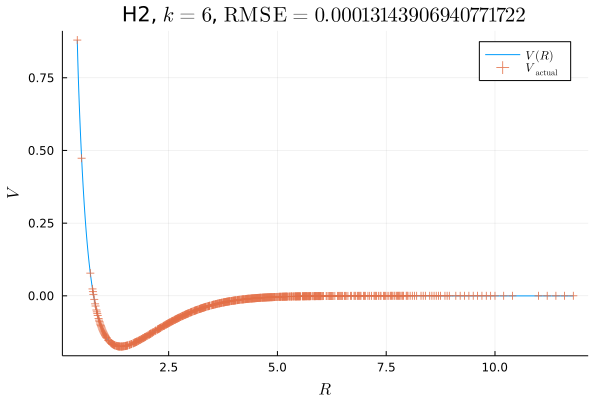
\includegraphics[scale=0.7]{img/linear_RATPOT/linratpot_fit_H2_example.png}
    \caption{Nonlinear leastsquares fitting applied for linear RATPOT.}
    \label{fig:linratpot_fit}
\end{figure}

\begin{figure}[H]
    \centering
    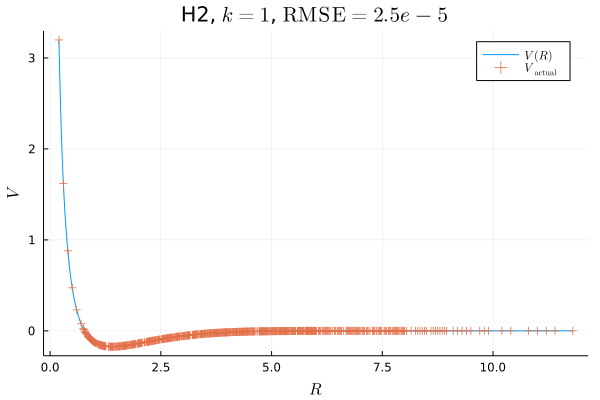
\includegraphics[scale=0.7]{img/linear_RATPOT/linratpot_linsolve_H2_example3.png}
    \caption{Directly solving linear RATPOT.}
    \label{fig:linratpot_linsolve}
\end{figure}


\subsection{Fitting method}
There exist several possible objective function forms which can be used to fit the diatomic functional forms. One possible objective function form is the RMSE in Eq.(\ref{eq:rmse}); another one would be the sum of squared residuals
\begin{equation}
    \sum^n_{i=1}\left[V(R_i) - V_{i,\text{ab initio}}\right]^2.
    \label{eq:sumsquaredresidual}
\end{equation}
There are two types of optimization routines for nonlinear least squares form, one requires the objective function to return a residual vector, another one is the standard optimization routine which requires the objective function to return a scalar. In the case of overdetermined system (more data than tuning parameters), \textbf{Levenberg-Marquardt} (LM) algorithm \cite{lm} is employable; otherwise, local search such as \textbf{trust region reflective} (TRF) \cite{trf} and \textbf{dogleg} algorithm with rectangular trust regions \cite{dogbox} are employable. This rule is molecule-size-agnostic, i.e., applicable to any molecule size.

\subsubsection{Fitting dissociated energy}
For any functional form of potential energy, it is possible to scale the curve in a way that the repulsive and attractive part of the potential curve is more visible. This is done by scaling both the functional form and the data by the dissociation energy
\begin{equation}
    \Delta = V_l - V_{\min},
    \label{eq:diss_energy}
\end{equation}
where $V_l$ is the potential energy at the largest distance and $V_{\min}$ is the minimum observed potential energy. This is done during the fitting (also applies to direct solvers):
\begin{equation}
    \theta_{\min} = f(V_\text{ab initio} / |V_\text{ab initio}| + \Delta, V(R) / |V(R)| + \Delta),
    \label{eq:diss_solve}
\end{equation}
where $\theta_{\min}$ is a vector containing optimized tuning parameters, here $f$ is an objective function for data-fitting, for example (\ref{eq:sumsquaredresidual}); and $V(R)$ is the functional form. Similarly, an adjusted RMSE for dissociated energy is
\begin{equation}
    \text{aRMSE} := \Delta \text{RMSE}(\delta),
    \label{eq:aRMSE}
\end{equation}
where
\begin{equation}
    \delta := \epsilon /(|V|+\Delta),
    \label{eq:delta}
\end{equation}
and
\begin{equation}
    \epsilon = V_\text{ab initio} - V(R).
    \label{eq:eps}
\end{equation}
\begin{figure}[htbp]
    \centering
    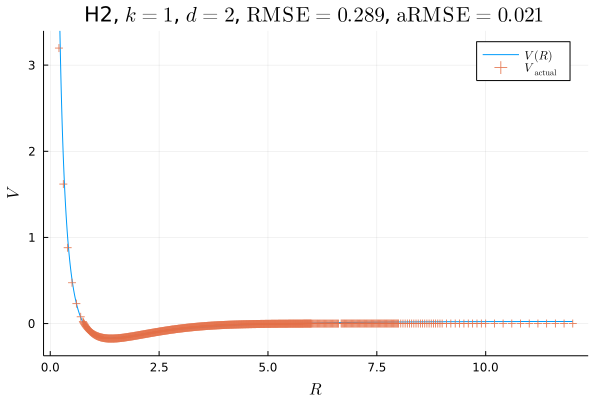
\includegraphics[scale=0.7]{img/linear_RATPOT/linratpot_linsolve_H2_val-end.png}
    \caption{Direct linear solve for linear dissociated RATPOT with 5 initial data points and 5 end data points as validation data.}
    \label{fig:linratpot_diss_linsolve}
\end{figure}

\iffalse
\section{Multivalued fit}
This is the new/innovative mathematical formula.
The multi-fit with just one formula, by making use of eigenvalue....


\begin{equation}
    \begin{split}
        y_l = \lambda_{kl}(x_l, \theta) + .... \\
        F_l(\theta) = 1/\sum_k 1/(y_l - \lambda_k(x_l, \theta)) \\
        \text{min} \sum F_l(\theta)^2.
    \end{split}
\end{equation}

\section{Many-body potential}
\begin{equation}
    V = \sum_i V_i + \sum_{i<j}\frac{Z_{ij}}{R}p_{ij} - \sum_{i<j}(\frac{R}{q_{ij}})^2
\end{equation}

\section{(placeholder) Conical Intersections}
Here is a family of symmetric 3 x 3 matrices with a conical intersection; a 3D plot of the three sheets of the surface of eigenvalues would be nice for the lecture.
\begin{equation}
    A(s,t)=
    \begin{pmatrix}
        t & 2t+s & t+1 \cr 2t+s & 2t & t+1 \cr t+1 & t+1 & t+1-s
    \end{pmatrix}
\end{equation}
The conical intersection is at $(s,t)=(2,-1)$ where the matrix becomes diagonal with a double eigenvalue.
\fi

\section{High-level summary of potentials with bonding features}
Several bonding features and models are applied for H$_3$ molecule. Each feature is a basis function, each model is composed of the combinations of multiplications and summations of several basis functions with different polynomial degrees and wrapped in several forms which are then multiplied by tuning coefficients.
\subsection{Features}
\subsubsection{Bonding function}
\label{subsub:bondingfunction}
The bonding function $b$ is formed by the \textbf{Chebyshev polynomials} which defines the polynomial degree of the \textbf{bond strength}. The bond strength is a piecewise continuous smooth function which transforms each diatomic distance depending on a lower bound cut off and an upper bound cut off parameters, if the distance is below the lower bound cut off parameter then the bond strength is constant, if the distance is in between the lower and upper bound cut off parameters then the bond strength is equal to some smooth function, otherwise the bond strength is $0$. Bonding function $b$ is relevant for almost all of the features used, the only exception is the \textbf{reference energy} feature.

Given a total number of atoms $n_{\text{atom}}$ (which implies degree of freedom $f_{\text{free}} := 0.5(n_{\text{atom}}^2 - n_{\text{atom}})$), polynomial degree $d_{\text{deg}}$, and total number of data points $n_{\text{data}}$, the bonding function is collected in an array with $(d_{\text{deg}}, f_{\text{free}}, n_{\text{data}})$ shape.

\subsubsection{Reference energy}
\label{subsub:referencenergy}
The \textbf{reference energy} $U$ is a diatomic energy function which sums each energy of the possible combinations of the diatomic distances. For each atom $i$, it is the sum of energies of all of the possible distances which includes atom $i$, this depends on the degree of freedom of the molecule. For example, for triatomic molecules, the reference energy of each atom is composed of 2 terms of diatomic energy function to be summed; as a concrete example, for $i=1,2,3$, then $U := ( U[1] := V(R_{12}) + V(R_{13}), U[2] := V(R_{21}) + V(R_{23}), U[3] := V(R_{31}) + V(R_{32}) )$. Since diatomic distance is permutationally invariant, then $R_{ij} = R_{ji}$, which means the indices can be re-arranged into $\{[(1,2), (1,3)], 
[(1,2), (2,3)],
[(1,3), (2,3)]\}$, this type of indexing would be more efficient given ordered vector of distances $\mathbf{R}$, since it is possible to map each tuple of distance index into a scalar index, which needs only to be computed once at the beginning. Since for each atom $i$, $U[i]$ sums the diatomic energies which depend on the degree-of-freedom indices, then given $n_{\text{atom}}$ and $n_{\text{data}}$, $U$ is an array with $(n_{\text{atom}}, n_{\text{data}})$ shape. This indexing rule is, in fact, applicable to any molecule with $n_{\text{atom}} > 2$. 

The reference energy has various diatomic terms depending on the model (the models will be explained in later sections). For model with trainable reference pair potential, for each atom, the diatomic energy function is similar to the bond strength function in Section \ref{subsub:bondingfunction}, it is a non-smooth non-continuous function depending on a lower bound cut off parameter and upper bound cut off parameter. For model with fixed H$_2$ contribution, it uses a smooth and continuous rational polynomial function where the denominator has at least degree 6. 


\subsubsection{Coordination vector}
For atom $i$, the \textbf{coordination vector} $Y[i] = (Y_1[i], Y_2[i], ..., Y_{d_{\text{deg}}}[i])$, is the sum of bonding function for atom $i$ where the summation indices are equal to the summation indices of the reference energy in Section \ref{subsub:referencenergy}. All components of $Y[i]$ are invariant under translation, rotation, and reflection due to each being the sum of the degree of freedom of each atom. When considering all atoms, $Y$ is an array with $(n_{\text{atom}}, d_{\text{deg}}, n_{\text{data}})$ shape.

\subsubsection{Orientation vector}
The \textbf{orientation vector} $r[i] = (r_1[i], r_2[i], ..., r_{d_{\text{deg}}}[i])$ is the sum of the multiplication between bonding function and difference of two atomic coordinates; similar to the previous section, the summation uses the indexing rule in Section \ref{subsub:referencenergy}. However this does not imply complete invariant (translation, rotation, and reflection), due to the difference of two coordinates only represents translation invariant property; e.g., let $x_k$ be the atomic coordinate of atom $k$ in three-dimensional Cartesian coordinate system, then $x_i - x_j \neq x_j - x_i$, which breaks the rotation and reflection invariant properties. Given $n_{\text{data}}$, $d_{\text{deg}}$ and $f_{\text{free}}$ of the bonding function, the dimension of the coordinate from $x_k$ for all $k$ (which in molecular system case it is always $3$), and $n_{\text{atom}}$ obtainable from the indexing routine, then $r$ is an array with $(n_{\text{atom}}, d_{\text{deg}}, n_{\text{data}}, 3)$ shape.

Additionally, since the available \textit{ab initio} data points throughout the literatures usually only provides the tuples of vector of distances and energy $[(\mathbf{R}_1, V_1), ..., (\mathbf{R}_{n_{\text{data}}}, V_{n_{\text{data}}})]$, then it would be necessary to transform the distance vectors into coordinate matrices whenever the coordinate matrices are not available from the data sources. 

\paragraph{Converting distances to coordinates}

\subparagraph{Algorithm.}
To calculate the Gram matrix $G$ with entries $G_{ik}:=x_i \cdot x_k$ in a coordinate system where the center of the mass is $0$, proceed as follows:
\begin{flalign}
    \quad q_{ik}:=r_{ik}^2, &&
    \label{eq:q}
\end{flalign}
\begin{flalign}
    \quad \gamma_i:=\frac{1}{N}\sum_k q_{ik}, &&
    \label{eq:gamma_i}
\end{flalign}
\begin{flalign}
    \quad \gamma:=\frac{1}{2N}\sum_i \gamma_i, &&
    \label{eq:gamma}
\end{flalign}
\begin{flalign}
    \quad G_{ii}=\gamma_i-\gamma, &&
    \label{eq:g_ii}
\end{flalign}
\begin{flalign}
    \quad G_{ik}=\frac12(G_{ii}+G_{kk}-q_{ik}), &&
    \label{eq:g_ik}
\end{flalign}
with $N$ defines the number of atom points.

Given $G$, calculate its eigenvalues and eigenvectors. Since $G$ is a positive semi definite matrix, all eigenvalues are non-negative, any near $0$ negative eigenvalue should be replaced by $0$. Finally, multiply the corresponding 3 eigenvectors by the square root of the corresponding eigenvalues. This defines the 3 components of the coordinate vectors $x_i$.

\subparagraph{Proof.}
The definition in (\ref{eq:q}) is required to be expanded in the terms of coordinates, it is written as
\begin{equation*}
    r_{ik}^2=(x_i-x_k)\cdot(x_i-x_k).
    \label{eq:q_expand}
\end{equation*}
Since the center of the mass is $0$, we have
\begin{equation*}
    \sum_k x_k = 0.
    \label{eq:centerofmass}
\end{equation*}
Here and later in this section, summations run over all atom points,
\begin{equation*}
    k = 1,..,N.
    \label{eq:k_index}
\end{equation*}
Using this, we find
\begin{equation*}
    \begin{split}
        \gamma_i &= \frac{1}{N} \sum_k q_{ik} = \frac{1}{N} \sum_k r_{ik}^2, \\
        &= \frac{1}{N} \sum_k (x_i-x_k) \cdot (x_i-x_k), \\
        %&= \frac{1}{N} \sum_k\left( x_i^2 - 2 x_i\cdot x_k + x_k^2 \right), \\
        &= \frac{1}{N} \left( \sum_k x_i^2 - \sum_k 2 x_i\cdot x_k + \sum_k x_k^2 \right), \\
        &= \frac{1}{N} \left( N (x_i^2) - 2 x_i \cdot \sum_k x_k + \sum_k x_k^2 \right), \\
        %&= \frac{1}{N} \left( N (x_i^2) + \sum_k x_k^2 \right), \\
        &= x_i^2 + \frac{1}{N}\sum_k x_k^2, \\
        \gamma &= \frac{1}{2N}\sum_i \gamma_i, \\
        %&= \frac{1}{2N} \sum_i \left( x_i^2 + \frac{1}{N} \sum_k x_k^2 \right), \\
        &= \frac{1}{2N}  \sum_i x_i^2 + \frac{1}{2N^2} N \sum_k x_k^2, \\
        %&= \frac{1}{2N}  \sum_i x_i^2 + \frac{1}{2N} \sum_k x_k^2, \\
        &= \frac{1}{N} \sum_k x_k^2.
    \end{split}
    \label{eq:gamma_i_expand}
\end{equation*}
\iffalse
We assume that all summations run over all points ($N$ atom points), i.e.,
\begin{equation}
    k = 1,..,N;
    \label{eq:k_index}
\end{equation}
by the distributivity of summation
\begin{equation}
    \sum_k c f(k) = c \sum_k f(k),
    \label{eq:distsum}
\end{equation}
and summation property
\begin{equation}
    \sum_k i = i \sum_k 1 = iN,
    \label{eq:sumdiff}
\end{equation}
\fi
%Next, we proceed by expanding (\ref{eq:gamma}) using (\ref{eq:gamma_i_expand}):
\iffalse
\begin{equation}
    \begin{split}
        \gamma &= \frac{1}{2N}\sum_i \gamma_i, \\
        %&= \frac{1}{2N} \sum_i \left( x_i^2 + \frac{1}{N} \sum_k x_k^2 \right), \\
        &= \frac{1}{2N}  \sum_i x_i^2 + \frac{1}{2N^2} N \sum_k x_k^2, \\
        %&= \frac{1}{2N}  \sum_i x_i^2 + \frac{1}{2N} \sum_k x_k^2, \\
        &= \frac{1}{N} \sum_k x_k^2.
    \end{split}
    \label{eq:gamma_expand}
\end{equation}
\fi
%then, by substituting the terms in (\ref{eq:g_ii}) using (\ref{eq:gamma_i_expand}) and (\ref{eq:gamma_expand}), we have
Therefore
\begin{equation*}
    G_{ii} =\gamma_i-\gamma = x_i^2 + \frac{1}{N}\sum_k x_k^2 - \frac{1}{N}\sum_k x_k^2 = x_i^2
    \label{eq:g_ii_proof}
\end{equation*}
%therefore
validates (\ref{eq:g_ii}). Using this we find
\iffalse
\begin{equation}
    G_{ii} = \gamma_i - \gamma \implies G_{ii} = x_i^2
    \label{eq:implication_g_ii}
\end{equation}
is true.
Since Eq.(\ref{eq:implication_g_ii}) is true, now we can show
\begin{equation}
    G_{ik} = \frac12(G_{ii}+G_{kk}-q_{ik}) \implies G_{ik} = x_i^Tx_k = x_i \cdot x_k
    \label{eq:g_ik_implication}
\end{equation}
is also true. 
Since (\ref{eq:implication_g_ii}) is true, then we can use (\ref{eq:q}) and (\ref{eq:g_ii_proof}) to rewrite (\ref{eq:g_ik}) into
\fi
\begin{equation*}
    \begin{split}
        G_{ik} &= \frac12(x_i^2 + x_k^2 - (x_i - x_k) \cdot (x_i - x_k))
        %&= \frac12(x_i^2 + x_k^2 - (x_i^2 - 2x_i \cdot x_k + x_k^2)), \\
        = x_i \cdot x_k    
    \end{split}
    \label{eq:g_ik1}
\end{equation*}
which validates (\ref{eq:g_ik}).

\subsubsection{Gram matrix}
For each atom $i$, \textbf{Gram matrix} $G[i]$ is a symmetric and positive semidefinite matrix formed by the dot product of the orientation vectors. As a feature, it is invariant to translation, rotation, and reflection. Given $n_{\text{atom}}$, $n_{\text{data}}$, and orientation vectors with maximum polynomial degree of $d_{\text{deg}}$, then $G$ is collected in an array with 4 indices with $(n_{\text{atom}}, d_{\text{deg}}, d_{\text{deg}}, n_{\text{data}})$ shape.

\subsubsection{Neighbourhood matrix}
In the case of triatomic systems, the neighbourhood matrix $\Theta[i]$ is the Gram matrix $G[i]$ subtracted by the two-body terms, hence the neighbourhood matrix only represents the three-body terms. Programmatically, the shape of $\Theta$ is equal to the shape of $G$.


\subsection{Models}
There are two types of model employed for H$_3$ molecule, one model makes use of trainable reference pair potential, and the other uses fixed H$_2$ contribution. All of the models employ the previously mentioned features (basis functions) as monomials. Each feature is collected in $\Phi = \Phi(U, Y, H)$, where $H$ is chosen either $G$ or $\Theta$ for each model. For example, for the vector of basis functions up to degree 1: $\Phi(1) = (U, Y_1)$, for basis functions up to degree 2: $\Phi(2) = (UY_1, Y_1^2, Y_2, G_{11})$; then these vectors of basis functions of different degrees of polynomials are arranged in a contiguous way within a single vector $\Phi = (U, Y_1, UY_1, Y_1^2, Y_2, G_{11},...)$. For H$_3$ molecule, there exists a total of 59 basis functions for all of the combinations of monomials up to degree 5. Programmatically, given $n_{\text{atom}}$, $n_{\text{data}}$, and total number of basis functions $n_{\text{basis}}$, the shape of array $\Phi$ is $(n_{\text{atom}}, n_{\text{basis}}, n_{\text{data}})$.


\subsubsection{Model with trainable reference pair potential}
\label{subsub:trainablepair}
For the $U$ monomial, this model uses a non-continuous non-smooth piecewise function with lower bound and upper bound cut off tuning parameters similar to the bonding function. There are a total of 7 tuning parameters from the bonding function and the $U$ monomial combined, collected in a vector $\rho := (\rho_1, \rho_2, ...\rho_7)$, where $\rho_2 \leq \rho_3 \leq ... \leq \rho_7$ relations need to be satisfied. 

The potential energy of the molecular system is the sum of all atomic energies, each atomic energy is composed of $3$ different partial energy terms, and each partial energy term is in the form of rational potential where each of the numerator and denominator has $n_{\text{basis}}$ tuning coefficients; in total there are $6 \times n_{\text{basis}}$ tuning coefficients for this model. For H$_3$ molecule, there is a maximum of $59$ basis functions (where $H = G$, up to $5$ degree of monomial combinations), this results in $6 \times 59 + 7 = 361$ tuning parameters.


\subsubsection{Model with fixed H$_2$}
In this model, a smooth and continuous rational potential function which has a polynomial of at least degree 6 in the denominator is used for the $U$ monomial with fixed parameters. The differences with the model in Section \ref{subsub:trainablepair} are, each atomic energy now is also summed with $U$; the numerator of each partial energy term now has $2 \times n_{\text{basis}}$ tuning coefficients; and the number of partial energy terms can be increased by adding more elementary terms to each of the partial energy term. Here $H = \Theta$ with a total of $64$ basis functions up to polynomial degree of $6$, hence a total of at least $9 \times 64 + 3 = 579$ tuning parameters overall are present.


\subsection{Objective function}
The objective function has the form of nonlinear least squares. The objective function considers the possibility of fitting multiple different datasets at once, this is compensated by the addition of two tuning parameters for each nonlinear least squares associated to a particular dataset: energy shift $\mu$ and the order of accuracy $\sigma$. 

In case of the model with trainable pair potential in Section \ref{subsub:trainablepair}, the first $7$ tuning parameters $\rho$ are slightly changed to compensate the constraints, they become $\pi := (\pi_1 = \log(\rho_1)/20, \pi_2 = \log(\rho_2)/20, \pi_3 = \sqrt{\rho_3}, \pi_4 = \sqrt{\rho_4 - \rho_3}, \pi_5 = \sqrt{\rho_5 - \rho_4}, \pi_6 = \sqrt{\rho_6 - \rho_5}, \pi_7 = \sqrt{\rho_7 - \rho_6})$ as the input of the optimization routine; which is then inverted into $\rho := (\exp(20\pi_1), \exp(20\pi_2), \pi_3^2,\pi_4^2 + \rho_3, \pi_5^2+\rho_4, \pi_6^2+\rho_5, \pi_7^2+\rho_6)$ for the potential evaluation. For model with fixed H$_2$, the tuning coefficients of partial energy terms are scaled by the expected magnitude of $\Phi$.

\subsection{High level programming details}
To compute the bonding features for fitting PES (function evaluator), a wrapper function which takes in all of the tuning parameters alongside the hyperparameters, and computes all of the features in a certain order, which then returns the energy value at the final step is required. Suppose 
\mint{python}|V = f_pot_bond(R, X, rho, sigma)| 
\noindent is the function to evaluate the energy given a matrix of atomic distances $\textbf{R} \in \mathbb{R}^{n_\text{data} \times f_\text{free}}$, array of atomic coordinates $\textbf{X}$ with the shape of $(n_\text{data}, n_\text{atom}, n_\text{dim})$, parameter vector $\rho$, and hyperparameter vector $\sigma$; with a vector of energy $\textbf{V} \in \mathbb{R}^{n_\text{data}}$ as the returned quantity. The features (and sub features) within the function are computed in this order:
\begin{itemize}
    \item Reference energy $U$.
    \item Bond strength $b$ (sub feature for coordination vector $Y$).
    \item Coordination vector $Y$.
    \item Difference array $\Delta$ (sub feature for orientation vector $r$).
    \item Orientation vector $r$.
    \item Gram matrix $G$.
    \item Array of basis functions $\Phi$.
    \item Partial (atomic) energy term $\epsilon[i]$, which finally sums into the energy value.
\end{itemize}

Additionally, index computation is done pre-function evaluation once for each atomic system, this indexer is passed into the function evaluation as an input. Suppose that the indexing function is
\mint{python}|indexer = atom_indexer(n_atom)|
\noindent this returns the $n$-body indices of molecular system containing $n$-atoms, let it be stored in a matrix $D \in \mathbb{Z}^{n_\text{atom} \times n_\text{atom} - 1}$. For example, with $n_\text{atom} = 4$, the indexer has entries
\begin{minted}{python}
indexer =   [
                [1, 2, 3],
                [1, 4, 5],
                [2, 4, 6],
                [3, 5, 6]
            ]
\end{minted}
\noindent this is useful for vectorization of any arithmetic operations which make use the degree of freedom indices given an ordered vector of distances $\textbf{R}_k \in \textbf{R}, k=0,1,2,...n_\text{data}$, for example, for $4$-body terms summation (using the indexer in the example above): $V_k = \sum_{j \neq i} \textbf{R}_{k,i,j}$ can be represented by
\mint{python}|V = sum(R[:, indexer])|
\noindent This indexer allows computations on vectors of distances without needing to transform matrix of distances into an array of adjacency matrices with 0 at the diagonals (in graph-terms) with $(n_\text{data}, n_\text{atom}, n_\text{atom})$ shape, which in turn reduces the space complexity. The indexer is used in reference energy $U$, coordination vector $Y$, and orientation vector $r$.

\subparagraph{Reference energy $U$.}
First the function
\begin{minted}{python}
U = U_ref_energy(R, C, R_h, R_C, R_0, g)
\end{minted}
decides the diatomic energy value within certain ranges for each element of  $\textbf{R}$ matrix. This is done using a sub function containing simple switch-statement
\begin{minted}{python}
if R <= R_h:
    return infinity
else if R_h < R <= R_C:
    return some smooth function f(R, R_0, g)
else:
    return 0
\end{minted}
\noindent where $C, R_h, R_C, R_0 \in \rho$ and $g \in \sigma$, then let $V^\text{diatomic} \in \mathbb{R}^{n_\text{data} \times f_\text{free}}$ be the matrix containing all of the returned values from above sub function. Next, the degree of freedom of each $V^\text{diatomic}_k \in \mathbb{R}^{f_\text{free}}$ is summed by using the indexer (essentially reducing the $f_\text{free}$ index to $n_\text{atom}$), hence the array $U$ has $(n_\text{atom}, n_\text{data})$ shape.

\subparagraph{Bond strength $b$.}
The bond strength function
\begin{minted}{python}
b = bond_strength(R, d_deg, n_atom, R_up, R_m, R_low, e)
\end{minted}
\noindent computes the bond strength of each element of $\textbf{R}$ matrix, where $\overline{R}, R_m, \underline{R} \in \rho$ and $d_\text{deg}, e \in \sigma$. First $t_0$ is obtained from a function which computes a smooth functional (polynomial with at least degree 2 in each numerator and denominator)
\mint{python}|t_0 = f_t_R(R_m, R_up, R_low, e)|
\noindent then matrix $t \in \mathbb{R}^{n_\text{data} \times f_\text{free}}$ is computed using the same function by passing the matrix $\textbf{R}$ at the $R_m$ argument position. Both $t_0$ and $t$ are used for the bond strength computation, which is essentially a similar switch sub function as the reference energy $U$ (notice the slight differences of the inequality relations)
\begin{minted}{python}
if R < R_low:
    return 1
else if R_low <= R <= R_up:
    return t_0/(t+t_0)
else if R_up < R:
    return 0
\end{minted}
then the result is stored in $s \in \mathbb{R}^{n_\text{data} \times f_\text{free}}$ matrix. On the next step, the bond strength $s$ will need to be wrapped in the terms of polynomials so that $s$ can have different degree of powers, in order to do this, the polynomials are evaluated recursively in terms of Tchebyshev polynomials
\mint{python}|b = tchebyshev_pol(d_deg, s)|
\noindent hence $b$ is an array with $(d_\text{deg}, n_\text{data}, f_\text{free})$ shape.

\subparagraph{Coordination vector $Y$.}
The function for coordination vector $Y$ simply computes the sum of the bond strength $b$ by using the indexer in the same manner with the second half of $U$ computation. Hence $Y$ has the shape of $(n_\text{atom}, d_\text{deg}, n_\text{data})$.

\subparagraph{Difference array $\Delta$.}
The delta array $\Delta$ with shape $(n_\text{data}, f_\text{free}, n_\text{dim})$ (specifically in molecular systems, $n_\text{dim} = 3$ always) contains $\textbf{X}_{:,j} - \textbf{X}_{:,i}, i<j$, where $\textbf{X}$ with the shape of $(n_\text{data}, n_\text{atom}, n_\text{dim})$ is the matrix containing molecular coordinates. The loop goes over the $n_\text{atom}$ index hence this is sort of the "inverse" of the indexer, since this transforms $n_\text{atom}$ into $f_\text{free}$.

\subparagraph{Orientation vector $r$.}
To compute the orientation vector $r$, first  the (elementwise) array multiplication between the $(n_\text{data}, f_\text{free})$ indices of $b$ and $(n_\text{data}, f_\text{free}, 3)$ indices of $\Delta$ needs to be computed for $d=1,2..,d_\text{deg}$, then let the result be stored in an array $\eta$ with shape $(d_\text{deg}, n_\text{data}, f_\text{free}, 3)$. Finally $\eta$ is summed using the indexer rule, which the final result is stored in array $r$ with the shape of $(n_\text{atom}, d_\text{deg}, n_\text{data}, 3)$.

\subparagraph{Gram matrix $G$.}
For each atom $i=1,2, ... n_\text{atom}$, for each $d_1 = 1,2,... d_\text{deg}$, and for each $d_2 = 1,2,... d_\text{deg}$:
\mint{python}|G[i] = sum(r[i][d_1]*r[i][d_2], axis=-1)|
\noindent this means that the elementwise array multiplication is done on the $(n_\text{data}, 3)$ indices, then the last index is summed (denoted by axis = $-1$ argument), hence the last index disappears, this represents the dot product between vectors. In the end $G$ is an array with $(n_\text{atom}, d_\text{deg}, d_\text{deg}, n_\text{data})$ shape.

\subparagraph{Array of basis functions $\Phi$.}
The array $\Phi$ with shape $(n_\text{atom}, n_\text{basis}, n_\text{data})$, consists of basis functions which are composed of the feature array which have been calculated previously, simply
\mint{python}|phi = f_phi(U, Y, G)|
\noindent 
for each degree, all possible polynomials are enumerated, each polynomial is the combination of each feature array, for example
\begin{minted}{python}
# degree 1:
phi[:, 0] = U;
phi[:, 1] = Y[:, 0];

# degree 2:
phi[:, 2] = U*Y[:, 0];
phi[:, 3] = Y[:, 0]**2; phi[:, 4] = Y[:, 1]; phi[:, 5] = G[:, 0,0];

#degree 3:
...

\end{minted}
which shows that $\Phi = (U, Y_1, UY_1, Y_1^2, Y_2, G_{1,1}, ...)$.

\subparagraph{Atomic energy terms $\epsilon[i]$.}
The atomic energy terms $\epsilon[i]$ are the sums of partial energy terms, where the partial energy terms are smooth rational functionals which depend on the tuning parameter matrices $A, B, C \in \mathbb{R}^{2 \times n_\text{basis}}$. Technically each element of each tuning parameter vectors are multiplied by $\Phi_k$, in simpler terms
\begin{minted}{python}
f_partial_energy(E, Phi):
    V_part_mat = matrix((2,n_basis), type="real")
    for k=0,1,...,n_basis:
        V_part_mat[0][k] = E[0][k]*Phi[i][k]
        V_part_mat[1][k] = E[1][k]*Phi[i][k]
    V_part = f_smooth_rat(V_part_mat) # some smooth rational function
    return V_part
\end{minted}
where $A, B,$ or $C$ is an input argument in place of $E$. Then the partial energies are combined in a certain way, for example $\epsilon[i] = V_\text{part}(A) - \sqrt{V_\text{part}(B) - V_\text{part}(C)}$. Finally the total energy of the system is $V = \sum^{n_\text{atom}}_{i=1} \epsilon[i]$.


\subsection{Feature statistics}
The statistics of all features described within this section are displayed in Table \ref{tb:featstat_crandom} and Table \ref{tb:featstat_copt}. The features are used to compute the energy of $6032$ data points of H$_3$ dataset.

\begin{table}[!htbp]
\centering
\caption{Statistics of each feature per atom index using pre-optimization parameters.}
\label{tb:featstat_crandom}
\begin{tabular}{ccccc}
\toprule
feature[atom] &   max & min & mean &  std \\
\midrule
$U[1]$    &  2.481150e+24 &  7.461384e+22 &  6.254963e+23 &  5.593566e+23 \\
$U[2]$    &  2.435484e+24 &  4.340160e+22 &  5.548411e+23 &  5.030545e+23 \\
$U[3]$    &  1.682283e+24 &  5.973577e+21 &  2.307342e+23 &  2.703311e+23 \\
$Y[1]$    &  2.000000e+00 & -2.234326e-02 &  3.997134e-01 &  7.999023e-01 \\
$Y[2]$    &  2.000000e+00 & -8.430624e-02 &  3.992064e-01 &  7.997078e-01 \\
$Y[3]$    &  2.000000e+00 & -1.055023e-01 &  3.989212e-01 &  7.996413e-01 \\
$G[1]$    &  7.428453e-02 &  0.000000e+00 &  3.107268e-03 &  1.070428e-02 \\
$G[2]$    &  1.743001e+00 &  7.438274e-16 &  3.483051e-02 &  1.402622e-01 \\
$G[3]$    &  2.486132e+00 &  2.166612e-15 &  5.631022e-02 &  2.146574e-01 \\
$\Phi[1]$ &  3.969833e+25 & -1.901475e+22 &  3.286893e+23 &  1.990261e+24 \\
$\Phi[2]$ &  3.896758e+25 & -2.559325e+22 &  2.923480e+23 &  1.776411e+24 \\
$\Phi[3]$ &  2.691653e+25 & -7.797651e+20 &  1.213176e+23 &  8.457775e+23 \\
\bottomrule
\end{tabular}
\end{table}

\begin{table}[!htbp]
\centering
\caption{Statistics of each feature per atom index using post-optimization parameters, with RMSE $= 0.069$ across all H$_3$ data.}
\label{tb:featstat_copt}
\begin{tabular}{ccccc}
\toprule
feature[atom] &   max & min & mean &  std \\
\midrule
$U[1]$    &  1.450460e-276 & -2.679209e-278 &  3.114115e-277 &  0.000000 \\
$U[2]$    &  1.422420e-276 & -4.622908e-278 &  2.679955e-277 &  0.000000 \\
$U[3]$    &  9.601608e-277 & -6.980936e-278 &  6.897668e-278 &  0.000000 \\
$Y[1]$    &   1.999660e+00 &  -4.937911e-01 &   3.189007e-01 &  0.644286 \\
$Y[2]$    &   1.999115e+00 &  -4.923274e-01 &   2.960542e-01 &  0.580598 \\
$Y[3]$    &   1.999115e+00 &  -4.978102e-01 &   2.358900e-01 &  0.533017 \\
$G[1]$    &   4.256561e+00 &   0.000000e+00 &   3.034012e-01 &  0.463637 \\
$G[2]$    &   3.609277e+00 &   5.088141e-06 &   3.312816e-01 &  0.419666 \\
$G[3]$    &   5.362877e+00 &   2.099490e-06 &   4.990154e-01 &  0.741347 \\
$\Phi[1]$ &   3.197281e+01 &  -1.031954e+00 &   8.880903e-01 &  3.839208 \\
$\Phi[2]$ &   3.192923e+01 &  -1.024145e+00 &   6.708816e-01 &  3.008128 \\
$\Phi[3]$ &   3.192923e+01 &  -1.031435e+00 &   6.205682e-01 &  2.927580 \\
\bottomrule
\end{tabular}
\end{table}

\section{Primitive bonding features}
\subsection{Coordination function}
A spline-like $C^2$ function if $t^2<1$ and $0$ otherwise, in the form of
\begin{equation}
    z(t) = a - bt - ct^5 + dt^3,
    \label{eq:f_z}
\end{equation}
where $t \in \mathbb{R}$. The coordination function is formed by fulfilling these conditions:
\begin{equation}
    \begin{split}
        z(-1) = 1, \\
        z(1) = 0, \\
        z'(\pm 1) = 0, \\
        z''(\pm 1) = 0.
    \end{split}
    \label{eq:f_coord_cond}
\end{equation}
In order to obtain the correct $a, b, c, d$, the conditions in (\ref{eq:f_coord_cond}) need to be expanded, which results in a linear system of equations
\begin{equation}
    \begin{split}
        z(-1) = a + b + c - d = 1, \\
        z(1) = a - b - c + d = 0, \\
        z'(\pm 1) = -b -5c +3d = 0, \\
        z''(\pm 1) = 20c - 6d = 0.
    \end{split}
    \label{eq:f_coord_lineq}
\end{equation}
By solving (\ref{eq:f_coord_lineq}) and writing the coefficients explicitly for the $t^2 < 1$ condition, the coordination function is
\begin{equation}
    z(t) = 
    \begin{cases}
        1, & \text{if } t \leq -1 \\
        0, & \text{if } t \geq 1 \\
        \frac{1}{2}-t\left(\frac{15}{16}+s \left(\frac{3}{16}s -\frac{10}{16}\right)\right). & \text{if } s=t^2 < 1
    \end{cases}
    \label{eq:f_coord}
\end{equation}
(\ref{eq:f_coord}) can be verified by differentiating $z(t)$ directly and expanding the second last condition in (\ref{eq:f_coord_cond})
\begin{equation}
    \begin{split}
        &z'(t) = \frac{d}{dt}\left[ \frac{1}{2}-t\left(\frac{15}{16}+t^2 \left(\frac{3}{16}t^2 -\frac{10}{16}\right)\right)\right] = -\frac{15}{16}(t+t^4-2t^2), \\
        &z'(\pm 1) = 0.
    \end{split}
\end{equation}

\subsection{Bump functions}
The bump functions, has the form
\begin{equation}
    f_k(t) = (1-(t-k)^2)^3_+
    \label{eq:f_bump}
\end{equation}
where $k \in \mathbb{Z}$, is a $C^2$ function everywhere except when $t \geq k+1$ or $t \leq k-1$, in which $f_k$ is $0$. The transformed $r \in \mathbf{R}$ has the form of  
\begin{equation}
    t = c_{xy}(r^2 - r^2_{xy}),
    \label{eq:t_bump}
\end{equation}
where
\begin{equation}
    c_{xy} = \frac{N}{\bar{r}_{xy}^2 - \ubar{r}_{xy}^2}
    \label{eq:c_xy}
\end{equation}
is a coefficient which depends on the largest atomic distance $\bar{r}_{xy}^2$ and smallest atomic distance $\ubar{r}_{xy}^2$. While $r_{xy}$ itself denotes the equilibrium distance of xy atomic pair (i.e., the closest distance where $dV/dr \approx 0$), for example, $r_{\text{HH}} \approx 1.4172946$ Bohr.

From (\ref{eq:t_bump}) we can define the upper bound and lower bound of $t$ as
\begin{equation}
    \begin{split}
        \ubar{t} = c_{xy}(\ubar{r}_{xy}^2 - r^2_{xy}), \\
        \bar{t} = c_{xy}(\bar{r}_{xy}^2 - r^2_{xy}),
    \end{split}
    \label{eq:t_bounds}
\end{equation}
when $\bar{t}$ and $\ubar{t}$ are rounded to the nearest integers, this tells
\begin{equation}
    N = \bar{t} - \ubar{t},
    \label{eq:t_N}
\end{equation}
which is a hyperparameter that describes the number of the primitive functions needed to approximate the associated pair-potential. The list of required $k$ for the total number of $N-1$ bump functions $f_k$ can be obtained by
\begin{equation}
    k \in \mathbb{Z} \cap \ubar{t} < k <\bar{t}.
\end{equation}
\begin{figure}[H]
    \centering
    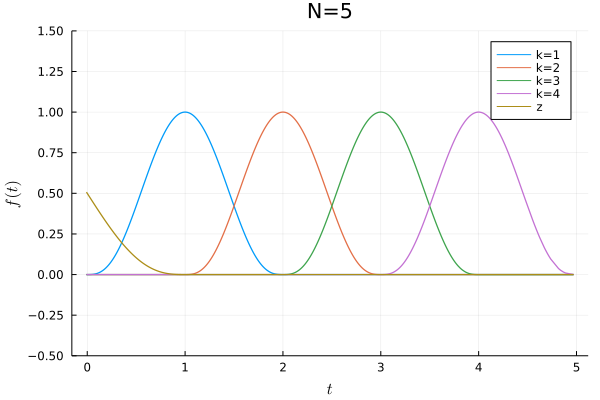
\includegraphics[scale=0.7]{img/zb(5).png}
    \caption{$z(t)$ and $f_k(t)$ for $k=1,2,...4$ computed from $\mathbf{R}_{:,3}$ of H$_3$ dataset.}
    \label{fig:zb(5)}
\end{figure}

\subsection{Linearizable bump functions}
Total params: $2N+2$.
Scaler:
\begin{equation}
    q := \frac{N}{1+\rho} \in (0,N]
\end{equation}
Basic bump:
\begin{equation}
    h_k := [1-(q-k)^2]^3_+
\end{equation}
Basis LC:
\begin{equation}
    u(q) = \sum_{k=0}^N(\theta_k (q-k) + \theta_{k+N+1})h_k
\end{equation}
Bumpsum:
\begin{equation}
    w(q) = \sum h_k
\end{equation}
Since most $h_k$ vanish:
\begin{equation}
    \begin{split}
        & i := \ceil{q} \geq 1, \\
        & \epsilon := i-q \in [0,1) \implies q = i - \epsilon \in (i-1,i]
    \end{split}
\end{equation}
Simplified expressions:
\begin{equation}
    \begin{split}
        & \alpha := (\epsilon(2-\epsilon))^3 \\
        & \beta := (1-\epsilon^2)^3
    \end{split}
\end{equation}
Simplified bump:
\begin{equation}
    h_k = 
    \begin{cases}
        \alpha & \text{ if }k=i-1, \\
        \beta & \text{ if }k=i, \\
        0 & \text{ otherwise }
    \end{cases}
\end{equation}
Simplified basis :C:
\begin{equation}
    u(q) = (\theta_i(q-i+1) + \theta_{i+N})\alpha + (\theta_i(q-i) + \theta_{i+N+1})\beta
\end{equation}
Simplified bumpsum:
\begin{equation}
    w(q) = \alpha + \beta
\end{equation}
Basic features:
\begin{equation}
    x := h_k(q)/w(q),
\end{equation}
\begin{equation}
    y := (q-k)h_k(q)/w(q)
\end{equation}
Linearized bumps:
\begin{equation}
    \begin{split}
        u(q) & = \sum \left(\frac{h_k(q)}{w(q)}\theta_k + \frac{(q-k)h_k(q)}{w(q)}\theta_{k+N+1}\right) \\
        & = A\theta = \sum A_{ik}\theta_k, \text{ if }q=q_i.
    \end{split}
\end{equation}

\begin{figure}[H]
    \centering
    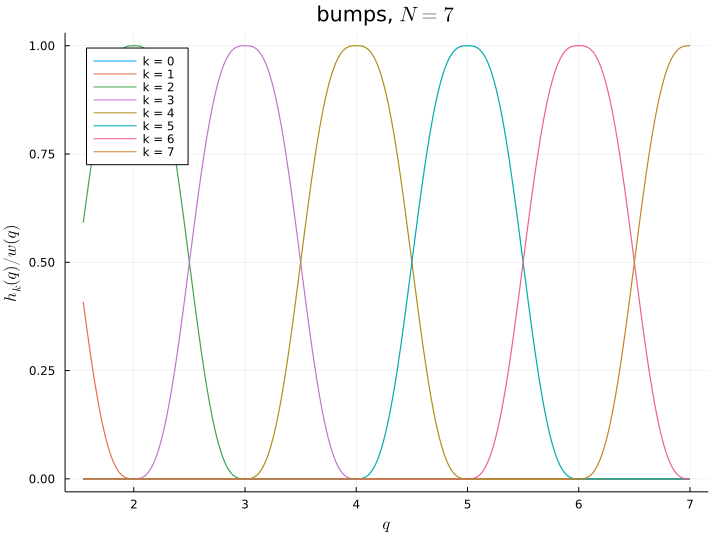
\includegraphics[scale=0.5]{img/BUMP/BUMP_hw_N=7.png}
    \caption{Bumps from $h_k(q)/w(q)$ for $N=7$.}
    \label{fig:linear_BUMP_x_N=7}
\end{figure}

\begin{figure}[H]
    \centering
    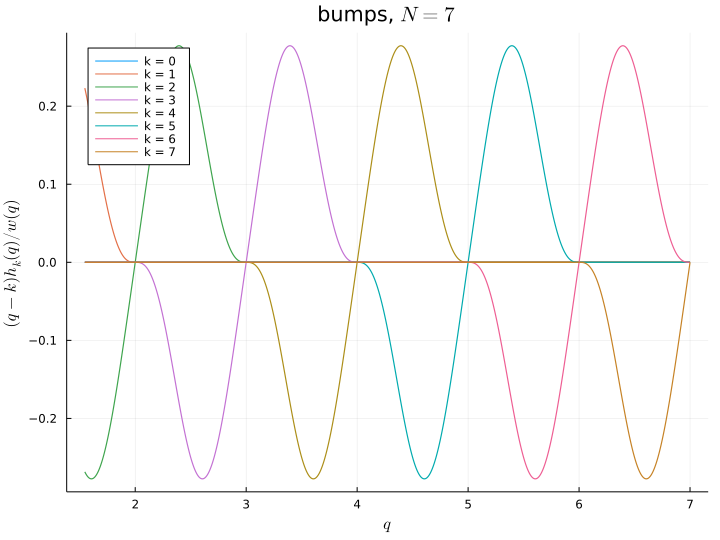
\includegraphics[scale=0.5]{img/BUMP/BUMP_qhw_N=7.png}
    \caption{Bumps from $(q-k)h_k(q)/w(q)$ for $N=7$.}
    \label{fig:linear_BUMP_y_N=7}
\end{figure}

\begin{figure}[H]
    \centering
    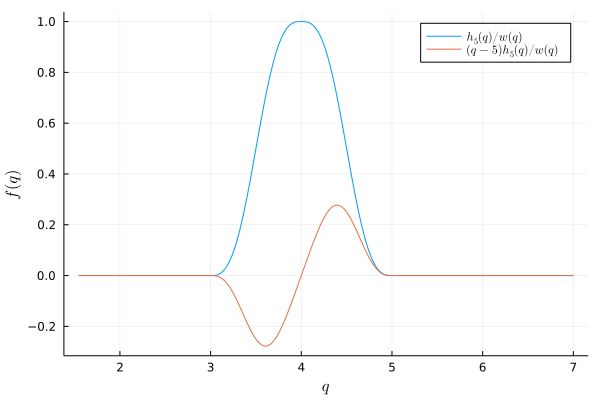
\includegraphics[scale=0.7]{img/BUMP/BUMP_k=5.png}
    \caption{Bumps for $x$ and $y$ when $k=5$.}
    \label{fig:linear_BUMP_k=5}
\end{figure}

\section{Datasets}
\subsection{H$_2$ data}
The data points for ground state H$_2$ (Figure \ref{fig:h2}) are obtained from \textsc{Hager-Roiser} \cite{ulrik}, it contains:
\begin{itemize}
    \item Data sizes:
    \begin{itemize}
        \item \textsc{Kolos \& Wolniewicz} (1965) \cite{idx166}: 87 data points.
        \item \textsc{Wolniewicz} (1993) \cite{idx167}: 670 data points.
    \end{itemize}
    \item The energy values of \textsc{Wolniewicz} (1993) are shifted by $V_i := V_i-V_{670}$, $i=1,2,...,670$, to accommodate the asymptotic energy $\lim_{R \to \infty} V(R) = 0$.
\end{itemize}
\subsubsection{H$_2^+$ data}
The H$_2^+$ datasets are obtained from \textsc{Sharp} (1971) \cite{idx172}, with the following information:
\begin{itemize}
    \item Data sizes:
    \begin{itemize}
        \item $X^2\Sigma_g^+ 1s \sigma_g$ state: 29 data points.
        \item $\sigma_g 1s$ state: 29 data points.
        \item $2p \sigma_u$ state: 29 data points.
        \item $\sigma_u 1s$ state: 29 data points.
    \end{itemize}
    \item The energy and distance units are converted from (Angstrom, eV) to (Bohr, Hartree).
    \iffalse
    \item $V_{25}$ of $\sigma_u 1s$ state is corrected by replacing it with $V_{25} := f(R_{25})$, where $f$ is a linear interpolation model formed by $(R_I,V_I)$, $I=\{24,25,26,28,29\}$ data points.
    \fi
    \item The data of $\sigma_u 1s$ state is corrected by removing the $(R_{25}, V_{25})$ data point.
    \item For each state, the data are shifted by the first ionization energy of H, $V_{\text{ion}} = 1312$ kj/mol.
    \item Only $X^2\Sigma_g^+ 1s \sigma_g$ and $2p \sigma_u$ states are used while $\sigma_g 1s$ and $\sigma_u 1s$ states are excluded due to redundancy.
\end{itemize}
\begin{figure}[htbp]
    \centering
    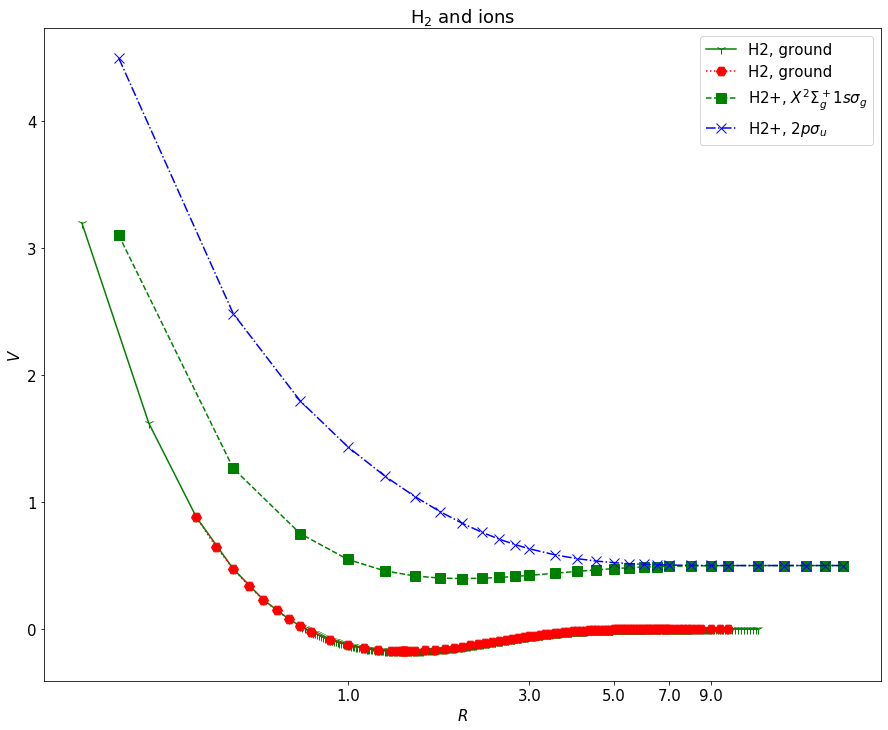
\includegraphics[scale=0.55]{img/H2_and_ions.png}
    \caption{Potential energy curves of H$_2$ and its ions.}
    \label{fig:h2}
\end{figure}


\iffalse %%%%%%%%%%%%%%%%%
\begin{figure}[h]
    \centering
    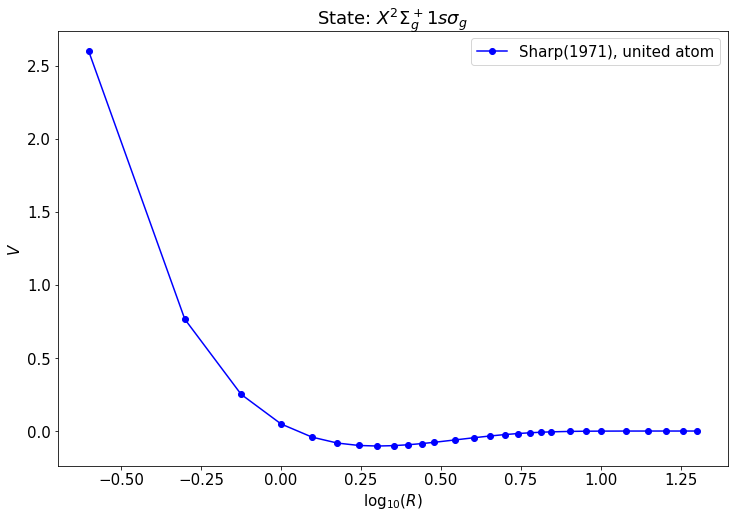
\includegraphics[scale=0.5]{img/H2plus_X2sigmagplus_Sharp(1971).png}
    \caption{Potential energy curve of H$_2^+$ for the $X^2\Sigma_g^+ 1s \sigma_g$ state.}
    \label{fig:h2+1}
\end{figure}
\begin{figure}[h]
    \centering
    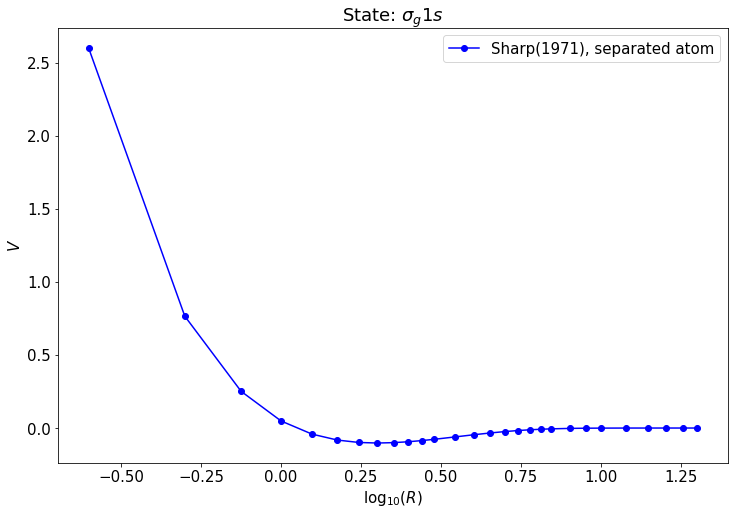
\includegraphics[scale=0.5]{img/H2plus_sigmag1s_Sharp(1971).png}
    \caption{Potential energy curve of H$_2^+$ for the $\sigma_g 1s$ state.}
    \label{fig:h2+2}
\end{figure}
\begin{figure}[h]
    \centering
    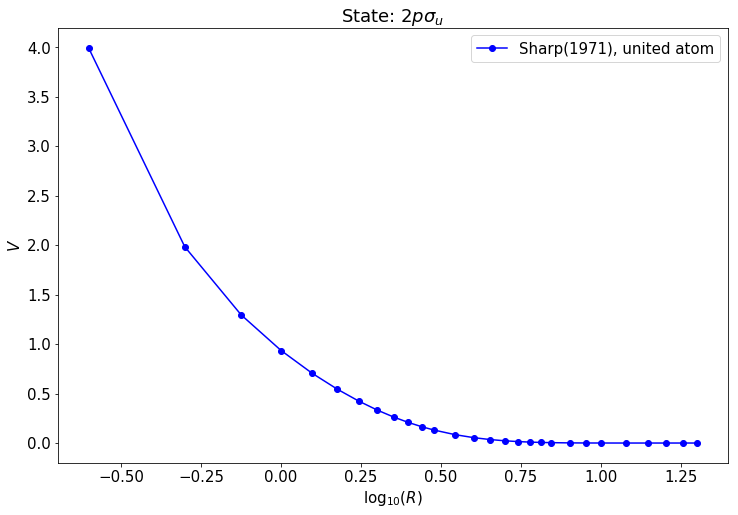
\includegraphics[scale=0.5]{img/H2plus_2psigmau_Sharp(1971).png}
    \caption{Potential energy curve of H$_2^+$ for the $2p \sigma_u$ state.}
    \label{fig:h2+3}
\end{figure}
\begin{figure}[h]
    \centering
    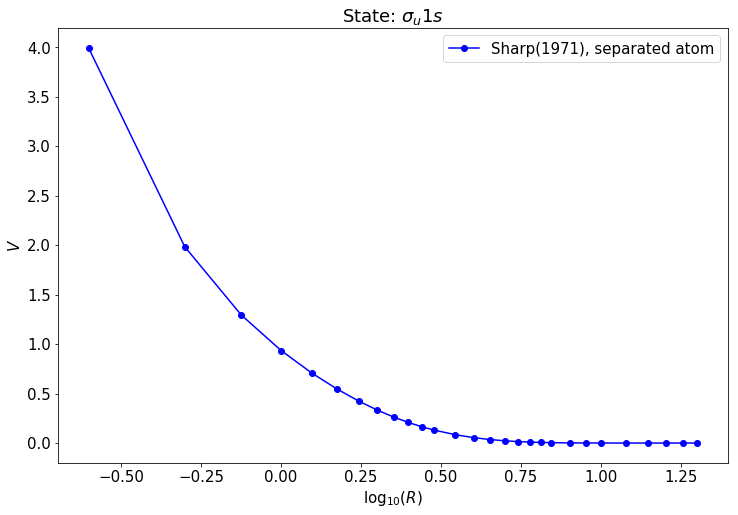
\includegraphics[scale=0.5]{img/H2plus_sigmau1s_Sharp(1971).png}
    \caption{Potential energy curve of H$_2^+$ for the $\sigma_u 1s$ state.}
    \label{fig:h2+4}
\end{figure}
\fi %%%%%%%%%%%%%%%%%%%%%%

\subsection{O$_2$ data}
The data points for O$_2$ (Figure \ref{fig:o2}) are provided by \textsc{Bytautas} et al (2010)\cite{idx158}, which describes:
\begin{itemize}
    \item Data sizes:
    \begin{itemize}
        \item $^3\Sigma^-_g$ state: 26 data points.
        \item $^1\Delta_g$ state: 26 data points.
        \item $^1\Sigma^+_g$ state: 26 data points.
    \end{itemize}
    \item The energy and distance units are converted from (Angstrom, millihartree) to (Bohr, Hartree) ($1$ Hartree $=$ $1000$ millihartree).
\end{itemize}
\subsubsection{O$_2^+$ data}
The data points for O$_2^+$ are provided by \textsc{Xavier} et al (2018) \cite{idx174}, the information contains:
\begin{itemize}
    \item Data sizes:
    \begin{itemize}
        \item $X^2\Pi_g$ state:
        \begin{itemize} 
            \item AV5Z method: 51
            \item AV6Z method: 51
            \item CBS method: 51
        \end{itemize}
    \end{itemize}
    \item The unit of $R$ is converted from Angstrom to Bohr.
    \item The $V$ is shifted by the first ionization energy of O, $V_{\text{ion}} = 1313.9$ kj/mol.
    \item Only one dataset is chosen due to the fact that each dataset is identical to each other (e.g., only the dataset from CBS method is picked).
\end{itemize}
\begin{figure}[h]
    \centering
    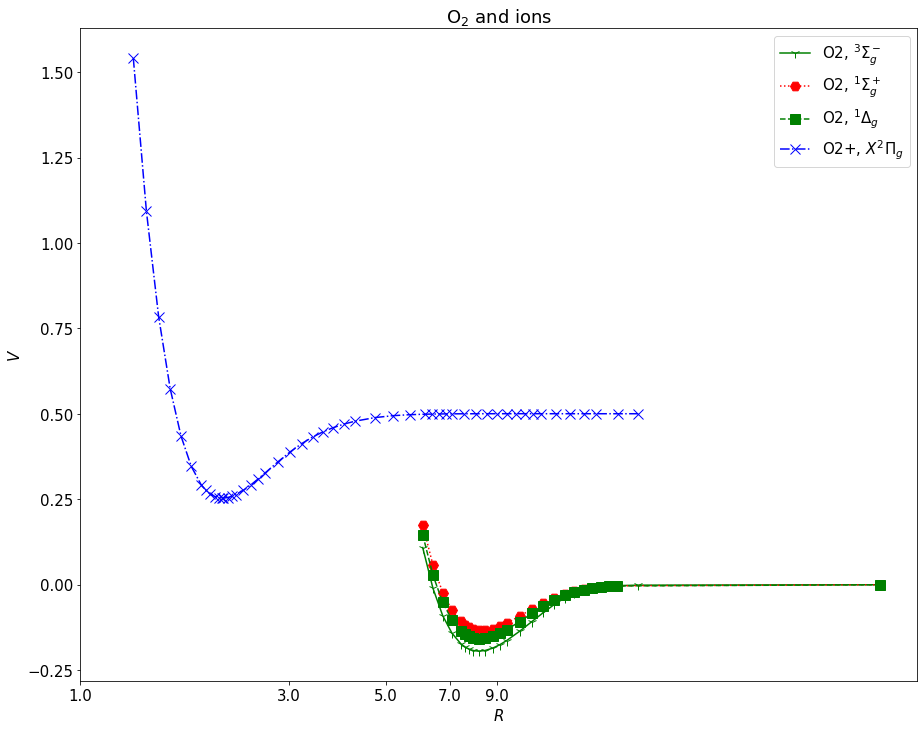
\includegraphics[scale=0.55]{img/O2_and_ions.png}
    \caption{Potential energy curves of O$_2$ and its ions.}
    \label{fig:o2}
\end{figure}


\iffalse %%%%%%%%
\begin{figure}[h]
    \centering
    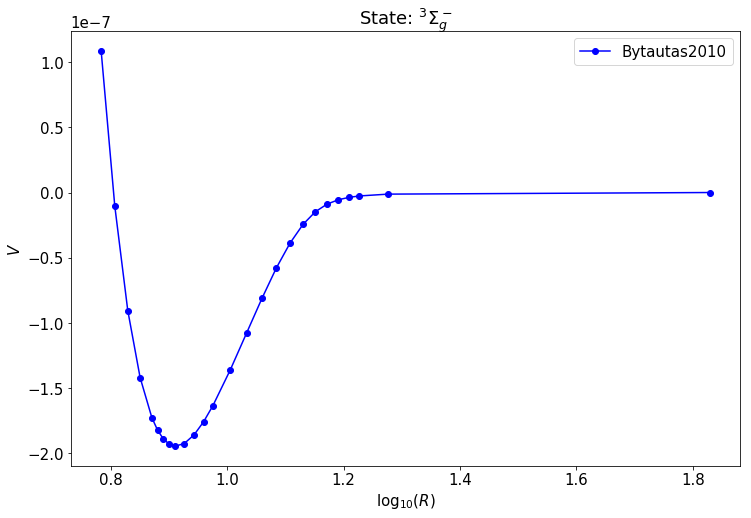
\includegraphics[scale=0.5]{img/O2_3sigmagminus_Bytautas(2010).png}
    \caption{Potential energy curve of O$_2$ for the $^3\Sigma^-_g$ state.}
    \label{fig:o21}
\end{figure}
\begin{figure}[h]
    \centering
    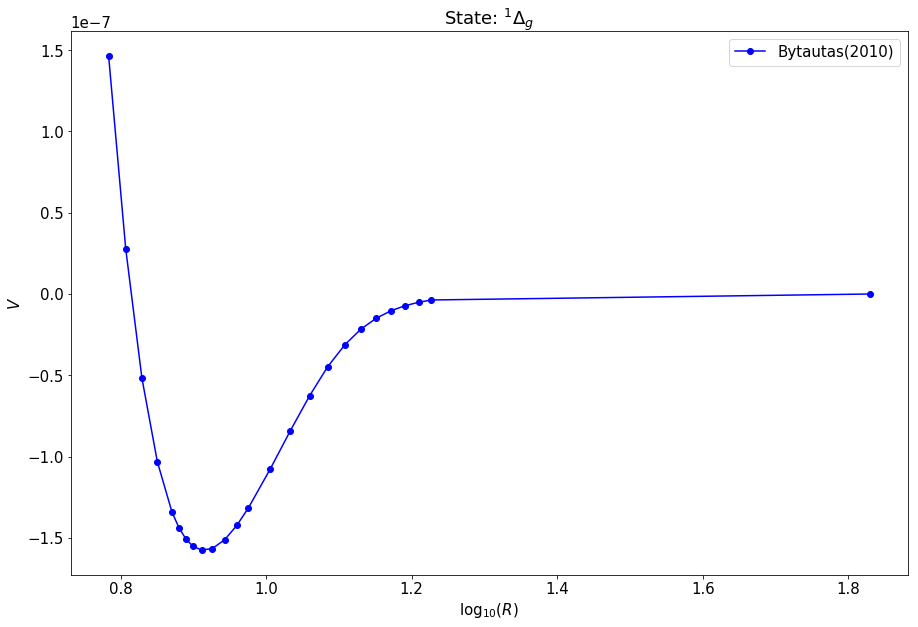
\includegraphics[scale=0.5]{img/O2_1deltag_Bytautas(2010).png}
    \caption{Potential energy curve of O$_2$ for the $^1\Delta_g$ state.}
    \label{fig:o22}
\end{figure}
\begin{figure}[h]
    \centering
    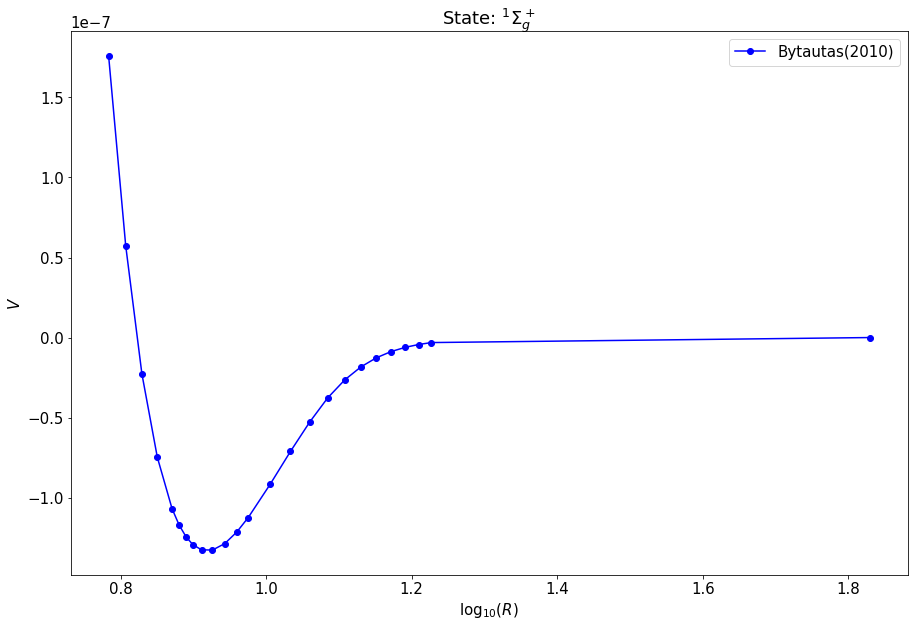
\includegraphics[scale=0.5]{img/O2_1sigmagplus_Bytautas(2010).png}
    \caption{Potential energy curve of O$_2$ for the $^1\Sigma^+_g$ state.}
    \label{fig:o23}
\end{figure}
\fi %%%%%%%%%%%%




\subsection{OH data}
The obtained OH datasets (Figure \ref{fig:oh}) are described by:
\begin{itemize}
    \item Data sizes:
    \begin{itemize}
        \item $X^2\Pi$ state:
        \begin{itemize}
            \item \textsc{Pradhan} (1995) \cite{idx163} (from \textsc{Shizgal} (1999) \cite{idx156}): 29 data points.
            \item \textsc{Nemukhin \& Grigorenko} (1997) \cite{idx160} (from \textsc{Shizgal} (1999) \cite{idx156}): 32 data points.
            \item \textsc{van Dishoeck et al} (1983) \cite{idx161} (from \textsc{Shizgal} (1999) \cite{idx156}): 24 data points.
            \item \textsc{Hodges} (1993) \cite{idx162} (from \textsc{Shizgal} (1999) \cite{idx156}): 32 data points.
            \item \textsc{Chu} et al (1974) \cite{idx159} using MCSCF method: 22 data points.
            \item \textsc{Chu} et al (1974) \cite{idx159} using CI method: 22 data points.
            \item \textsc{Werner} et al (1983) \cite{idx171}, using MCSCF-SCEP method: 17 data points.
            \item \textsc{Werner} et al (1983) \cite{idx171}, using SCEP-CEPA: 12 data points.
        \end{itemize}
        \item $A^2\Sigma^+$ state:
        \begin{itemize}
            \item \textsc{Chu} et al (1974) \cite{idx159}, using MCSCF method: 22 data points.
            \item \textsc{Chu} et al (1974) \cite{idx159}, using CI method: 22 data points.
        \end{itemize}
        \item $^4\Sigma^-$ state, obtained from \textsc{Shizgal} (1999) \cite{idx156}:
        \begin{itemize}
            \item \textsc{van Dishoeck \& Dalgarno} (1983) \cite{idx164}: 23 data points.
            \item \textsc{Hodges} (1993) \cite{idx162}: 23 data points.
            \item \textsc{Cooper} et al (1984) \cite{idx165}: 23 data points.
        \end{itemize}
        \item $^2\Sigma^-$ state, obtained from \textsc{Shizgal} (1999) \cite{idx156}:
        \begin{itemize}
            \item \textsc{Pradhan} (1995) \cite{idx163}: 21 data points.
            \item \textsc{van Dishoeck} et al (1983) \cite{idx161}: 14 data points.
            \item \textsc{Hodges} (1993) \cite{idx162}: 24 data points.
        \end{itemize}
        \item $^4\Pi$ state, obtained from \textsc{Shizgal} (1999) \cite{idx156}:
        \begin{itemize}
            \item \textsc{van Dishoeck \& Dalgarno} \cite{idx164}: 20 data points.
            \item \textsc{Hodges} (1993) \cite{idx162}: 20 data points.
            \item \textsc{Cooper} et al (1984) \cite{idx165}: 20 data points. 
        \end{itemize}
    \end{itemize}
    \item Data shifts:
    \begin{itemize}
        \item $V$ values for each dataset of \textsc{Chu} et al (1974) \cite{idx159} for $A^2\Sigma^+$ and $X^2\Pi$ states are shifted by its corresponding $V_n$.
        \item $V$ values on each dataset of \textsc{Werner} et al (1983) \cite{idx171} for $X^2\Pi$ state are shifted by its corresponding $V_n$.
    \end{itemize}
    \item Data corrections:
    \begin{itemize}
        \iffalse
        \item $V_1$ data of \textsc{Chu} et al (1974) \cite{idx159} for $X^2\Pi$ state is corrected by flipping its sign, $V_1 := -V_1$.
        \item $V_1$ data of \textsc{van Dishoeck \& Dalgarno} \cite{idx164} for $^4\Pi$ state is corrected by extrapolating $V_1 := f(R_1)$ where $f$ is a linear model built by $(R_I, V_I)$, $I=\{2,3,4\}$ data points.
        \item $V_4$ data of \textsc{van Dishoeck \& Dalgarno} \cite{idx164} for $X^2\Pi$ state is corrected by interpolating $V_4 := f(R_4)$ where $f$ is a linear model built by $(R_I, V_I)$, $I=\{2,3,5,6\}$ data points.
        \fi
        
        \item Data of \textsc{Chu} et al (1974) \cite{idx159} for $X^2\Pi$ state is corrected by removing $(R_1, V_1)$.
        \item Data of \textsc{van Dishoeck \& Dalgarno} \cite{idx164} for $^4\Pi$ state is corrected by removing $(R_1, V_1)$.
        \item Data of \textsc{van Dishoeck \& Dalgarno} \cite{idx164} for $X^2\Pi$ state is corrected by removing $(R_4, V_4)$.
    \end{itemize}
    \item The datasets used for fitting are:
    \begin{itemize}
        \item \{$X^2\Pi$, Pradhan(1995)\}.
        \item \{$X^2\Pi$, Nemukhin and Grigorenko(1997)\}.
        \item \{$X^2\Pi$, vanDishoeck et al(1983)\}.
        \item \{$^2\Sigma^-$, Pradhan(1995)\}.
        \item \{$^2\Sigma^-$, vanDishoeck et al(1983)\}.
        \item \{$^2\Sigma^-$, Hodges(1993)\}.
        \item \{$^4\Sigma^-$, vanDishoeck and Dalgarno(1983)\}.
        \item \{$^4\Sigma^-$, Hodges(1993)\}.
        \item \{$^4\Pi$, vanDishoeck and Dalgarno(1983)\}.
        \item \{$^4\Pi$, Hodges(1993)\}.
        \item \{$X^2\Pi$, Chu et al (1974)\}.
        \item \{$A^2\Sigma^+$, Chu et al (1974) \}.
        \item \{$A^2\Sigma^+$, Fallon et al(1960)\}.
    \end{itemize}
    \item Below datasets are excluded due to disagreeing with the majority of the datasets in the same molecular state:
    \begin{itemize}
        \item \{$^4\Sigma^-$, Cooper et al(1984)\}.
        \item \{$^4\Pi$, Cooper et al(1984)\}.
        \item \{$A^2\Sigma^+$, Chu et al (1974)\}.
        \item \{$X^2\Pi$,  Hodges(1993)\}.
        \item \{$X^2\Pi$, Werner et al(1983)\}.
        \item \{$X^2\Pi$, Chu et al (1974)\}.
    \end{itemize}
\end{itemize}
\subsubsection{OH$^+$ data}
The OH$^+$ data is obtained from \textsc{Werner} et al (1983) \cite{idx171} and \textsc{Xavier} et al (2018) \cite{idx174}, the contained information is:
\begin{itemize}
    \item Data sizes:
    \begin{itemize}
        \item $X^3\Sigma^-$ state:
        \begin{itemize}
            \item \textsc{Xavier} et al (2018) \cite{idx174}:
            \begin{itemize} 
                \item AV5Z method: 32
                \item AV6Z method: 32
                \item CBS method: 32
            \end{itemize}
            \item \textsc{Werner} et al (1983):
            \begin{itemize}
                \item MCSCF-SCEP method: 12 data points.
                \item SCEP-CEPA method: 12 data points.
            \end{itemize}
        \end{itemize}
    \end{itemize}
    \item The unit of \textsc{Xavier} et al (2018) \cite{idx174} $R$ is converted from Angstrom to Bohr.
    \item The $V$ values are shifted by the first ionization energy of O, $V_{\text{ion}} = 1313.9$ kj/mol.
    \item Only the datasets of \textsc{Xavier} et al \cite{idx174} with AV5Z method and \textsc{Werner} et al (1983) with SCEP-CEPA method are included, meanwhile the excluded datasets (in the form of \{state, author\}) are:
    \begin{itemize}
        \item \{$X^3\Sigma^-$, Werner et al(1983)\} due to disagreeing with other datasets.
        \item \{$X^3\Sigma^-$, Xavier(2018) - AV6Z method\} due to redundancy.
        \item \{$X^3\Sigma^-$, Xavier(2018) - CBS method\} due to redundancy.
    \end{itemize}
\end{itemize}

\subsubsection{OH$^-$ data}
The OH$^-$ data is obtained from \textsc{Werner} et al (1983) \cite{idx171}, the contained information is:
\begin{itemize}
    \item Data sizes:
    \begin{itemize}
        \item $X^1\Sigma^+$ state:
        \begin{itemize}
            \item MCSCF-SCEP method: 17 data points.
            \item SCEP-CEPA method: 10 data points.
        \end{itemize}
    \end{itemize}
\end{itemize}
\begin{figure}[h]
    \centering
    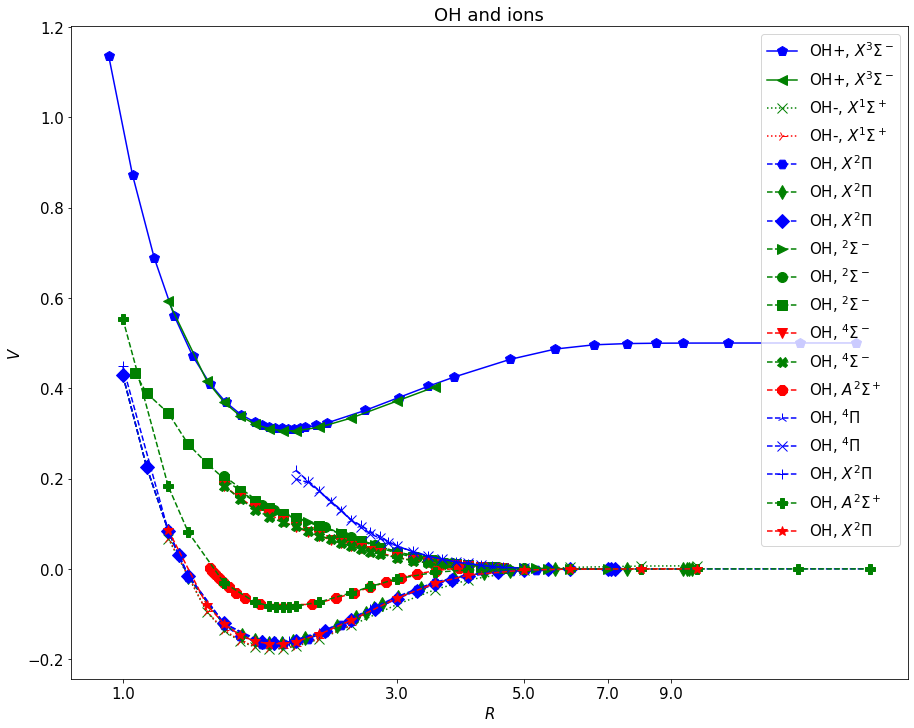
\includegraphics[scale=0.55]{img/OH_and_ions.png}
    \caption{Potential energy curves of OH and its ions.}
    \label{fig:oh}
\end{figure}

\iffalse
\begin{figure}[h]
    \centering
    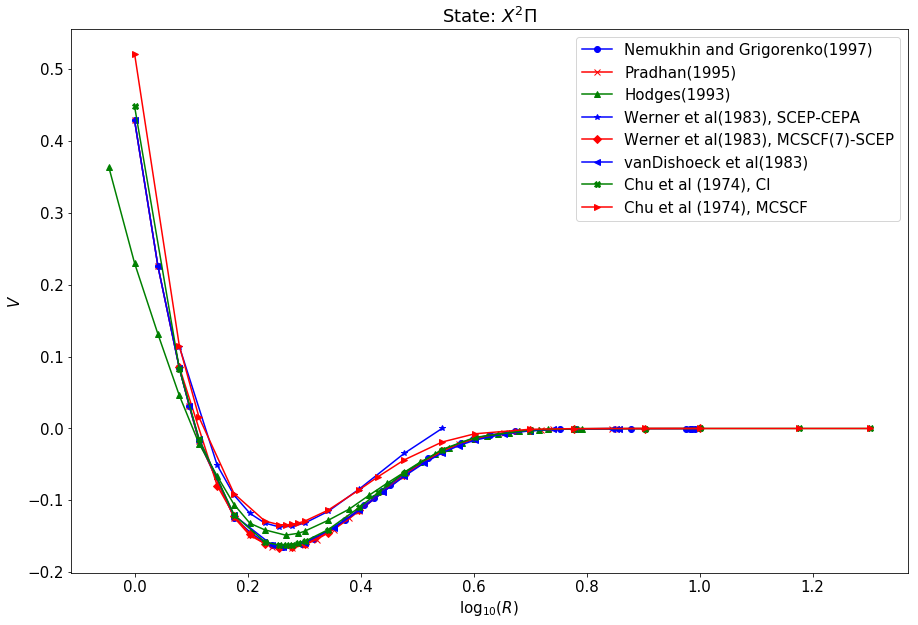
\includegraphics[scale=0.45]{img/OH_X2pi.png}
    \caption{Potential energy curve of OH for the $X^2\Pi$ state.}
    \label{fig:oh1}
\end{figure}
\begin{figure}[h]
    \centering
    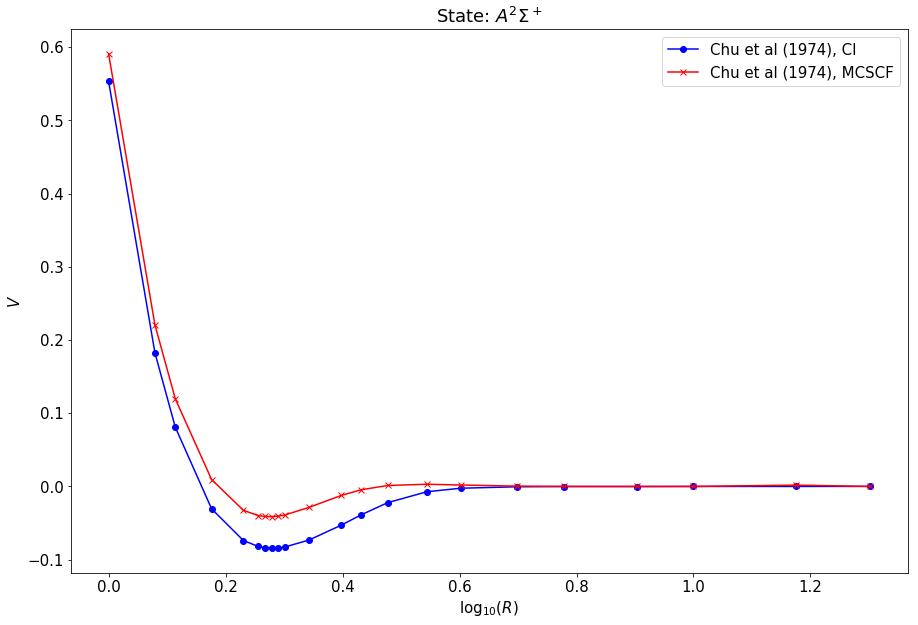
\includegraphics[scale=0.45]{img/OH_A2sigmaplus.png}
    \caption{Potential energy curve of OH for the $A^2\Sigma^+$ state.}
    \label{fig:oh2}
\end{figure}
\begin{figure}[h]
    \centering
    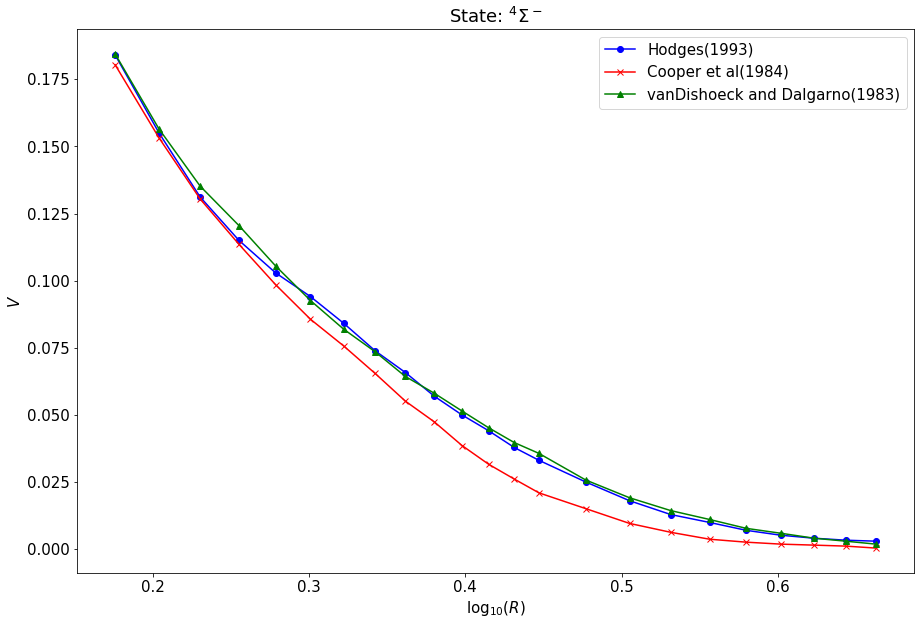
\includegraphics[scale=0.45]{img/OH_4sigmaminus.png}
    \caption{Potential energy curve of OH for the $^4\Sigma^-$ state.}
    \label{fig:oh3}
\end{figure}
\begin{figure}[h]
    \centering
    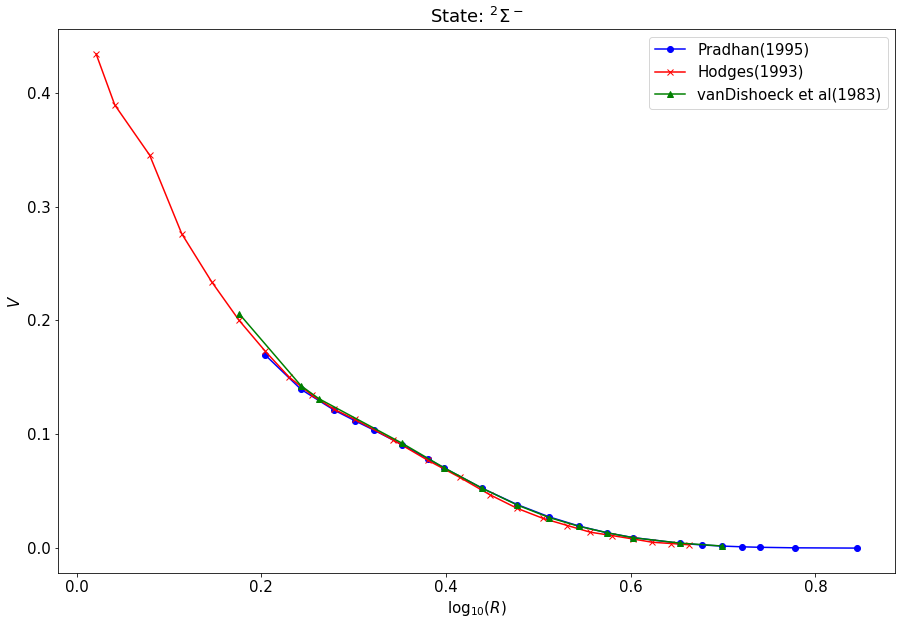
\includegraphics[scale=0.45]{img/OH_2sigmaminus.png}
    \caption{Potential energy curve of OH for the $^2\Sigma^-$ state.}
    \label{fig:oh4}
\end{figure}
\begin{figure}[h]
    \centering
    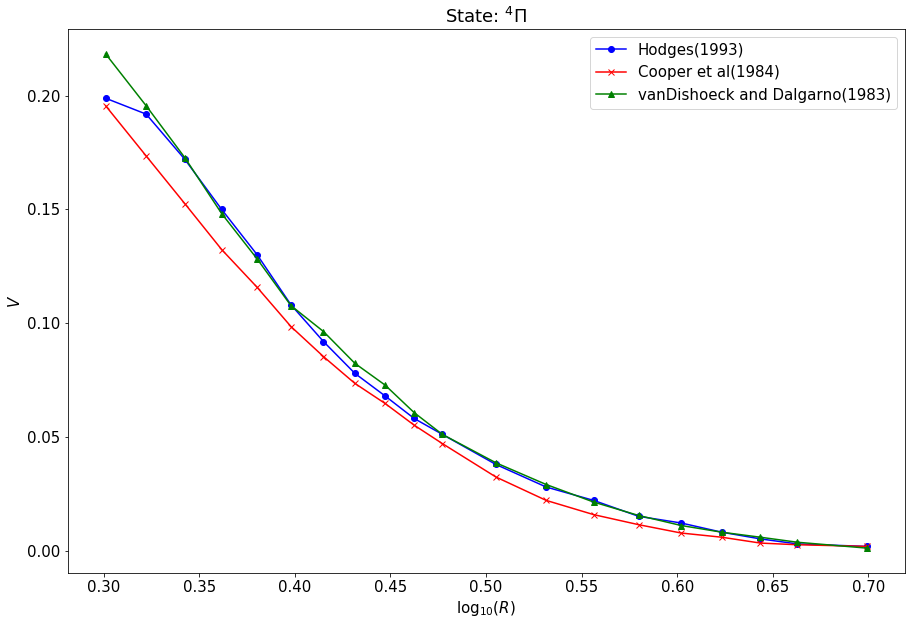
\includegraphics[scale=0.5]{img/OH_4pi.png}
    \caption{Potential energy curve of OH for the $ ^4\Pi$ state.}
    \label{fig:oh5}
\end{figure}
\fi








\clearpage
\bibliographystyle{unsrt}
\bibliography{sample}

\end{document}